\documentclass[dvipdfmx,openany]{jsbook}
\usepackage[dvipdfmx]{graphicx}                     % 画像表示
\usepackage{amsmath, amssymb, amsfonts, mathtools}  % 数式表示
\usepackage{amsthm}                                 % 定理表示
\usepackage[dvipdfmx]{hyperref}                     % 参考文献リンク
\usepackage{subcaption}                             % 小さいキャプション
\usepackage{url}                                    % url表示
\usepackage{enumerate}                              % 箇条書き
\usepackage{ascmac}                                 % 枠囲み
\usepackage{tcolorbox}                              % 枠囲み(プロンプト部分)
\usepackage{listings,jvlisting}                     % ソースコード表示
\usepackage{algpseudocode}                          % 疑似コード表示
\usepackage{algorithm}                              % アルゴリズム表示
\usepackage{booktabs}                               % 表の罫線
\usepackage{multirow}                               % 表のセル結合
\tcbuselibrary{breakable}
% \usepackage[dvipdfmx]{xcolor}                   % 参考文献リンク

\newcommand{\bhline}[1]{\noalign{\hrule height #1}}
\addtolength{\fullwidth}{-26truemm}  % 全体の幅(ヘッダ部の幅)を既定値から26mm小さくする
\setlength{\textwidth}{\fullwidth}   % 本文の幅(textwidth)を全体の幅(=ヘッダ部の幅)にそろえる
\setlength{\evensidemargin}{1truemm} % 偶数ページの左余白を1mm(+1インチ)にする
\setlength{\oddsidemargin}{19truemm} % 奇数ページの左余白を19mm(+1インチ)にする
\numberwithin{equation}{section}     % 式番号を(1.〇)で表示する
\setcounter{tocdepth}{2}             % subsubsectionまで目次に表示する

%%% ソースコード表示の設定 %%%
\lstset{
  basicstyle={\ttfamily},
  identifierstyle={\small},
  commentstyle={\smallitshape},
  keywordstyle={\small\bfseries},
  ndkeywordstyle={\small},
  stringstyle={\small\ttfamily},
  frame={tb},
  breaklines=true,
  columns=[l]{fullflexible},
  numbers=left,
  xrightmargin=0zw,
  xleftmargin=3zw,
  numberstyle={\scriptsize},
  stepnumber=1,
  numbersep=1zw,
  lineskip=-0.5ex
}
\renewcommand{\lstlistingname}{コード}

%%%% 表紙用設定 %%%%
\hoffset0mm
\voffset0mm
\makeatletter
\let\@@shipout\shipout
\def\shipout\vbox{\@@shipout\vbox\bgroup\afterassignment\insertBackGround\let\reserved@a=}
\def\insertBackGround#1{#1%
        \iftombow
                \copy\BackGround\kern0pt
        \else
                \kern-1truein\moveleft1truein\copy\BackGround\kern1truein
        \fi}
\newbox\BackGroundUnit
\newbox\BackGround
\def\@haikei#1{
\setbox\BackGroundUnit\hbox{\includegraphics*[width=\paperwidth]{#1}}
\@tempdima\paperheight
\advance\@tempdima\ht\BackGroundUnit\advance\@tempdima\dp\BackGroundUnit
\setbox\BackGround\vbox to \@tempdima{
        \@tempdima=\paperwidth\advance\@tempdima\wd\BackGroundUnit
        \leaders\hbox to\@tempdima{\leaders\copy\BackGroundUnit\hfil}\vfil
}
\wd\BackGround=0pt\ht\BackGround=0pt\dp\BackGround=0pt
}
\newcommand{\incluedefullgraphics}[1]{\pagestyle{empty}\@haikei{#1}\null}
\makeatother
%%%%%%%%%%%%%%%%%%%%

\begin{document}
\begin{titlepage}
  \thispagestyle{empty}
  \incluedefullgraphics{cover.png}
\end{titlepage}

\chapter*{はじめに}
本誌を手に取っていただき、ありがとうございます。
KaiRA会長の松田です。

\vskip\baselineskip

2022年11月のChatGPT公開以降、生成AIは驚異的なスピードで進化を遂げ、その普及は社会のあらゆる分野に広がっています。
現在では、文章だけでなく、画像、音声、さらには動画など、多様なデータ形式を扱える生成AIが次々と登場し、AI技術の社会実装がさらに加速しています。

\vskip\baselineskip

このような生成AIの開発には、高度な技術、膨大なデータセット、そして莫大な計算リソースが必要です。
そのため、多くの場合、大手企業や大学などの研究機関が主導する分野とされています。

\vskip\baselineskip

しかし、私たちは京都大学人工知能\textbf{研究会}の一員として、限られたリソースの中でも果敢に生成AIの開発に挑戦しました。
大規模プロジェクトには及ばない規模ではありますが、自ら手を動かして取り組むことで、生成AI技術の核心やその学習過程の困難さを直に体験し、多くのことを学ぶことができると信じています。

\vskip\baselineskip

夏休みから11月祭にかけて、私たちはオリジナルAIの開発プロジェクトを立ち上げました。
メンバー全員でアイデアを出し合い、試行錯誤を重ねながら、開発を進めてきました。
確かに、AIの学習には数多くの壁が立ちはだかり、必ずしも思い描いた成果を得るには至りませんでした。
しかし、それでも得られた経験と知見は非常に価値のあるものでした。

\vskip\baselineskip

本会誌では、私たちが試行錯誤しながら開発したオリジナルAIの挑戦と、その過程で得た教訓をご紹介します。
ぜひご一読いただき、私たちの取り組みをお楽しみいただけますと幸いです。

\vskip\baselineskip
\rightline{京都大学人工知能研究会KaiRA\ 会長}
\rightline{松田拓巳}
\rightline{2024年11月吉日}


\tableofcontents

\chapter{カメラ入力を用いた強化学習によるライントレーサの実現}\label{chap:line-tracer}
\section{はじめに}
DQN(Deep Q-Network\cite{mnih2013playing})の登場以降、強化学習は大きく発展し、これまでに様々な手法が提案されてきました。例えば、DreamerV3\cite{hafner2024masteringdiversedomainsworld}がマインクラフトにおいてダイヤモンドの採掘に成功するなど、ゲーム・シミュレーション分野では強化学習は一定の成功を収めています。しかしその一方で、実世界のロボットへの応用は未だに限定的と言えます。その理由はいくつかありますが、大まかに言えばシミュレーションと現実のギャップ、データ効率の問題、リアルタイム性の問題があります。それらの課題に対処するための研究も活発に行われており、模倣学習やモデルベース強化学習、オフライン強化学習やSim2Realなど、現在でも話題には事欠かない状態です。

この章では、実際に私が製作した強化学習で動作するライントレーサについて、その実装から結果までを説明します。

\section{全体像}
まず初めに、ライントレーサの全体像について述べます。このライントレーサのコンセプトは強化学習と全方向移動です。これら2つのコンセプトは互いに独立しているわけではなく、全方向移動が可能であることは強化学習にとってメリットとなっています。例えば非ホロノミックな対向二輪ロボットをベースに強化学習を行う場合、横方向には移動できないため、機体が向いている方向と、行動の関係を強化学習モデルに学習させる必要があります。一方で全方向移動が可能であれば、機体の方向に関わらず任意の方向に進めるため、学習難易度は低下します。

ライントレーサの外観は図\ref{fig:image1}のようになっています。透明な球殻の内部にオムニホイールを備えた本体が格納されており、球の重心の移動によって転がりながら動くような仕組みになっています。本体の底部中央にはWebカメラが設置してあり、それにより床面の様子を観測できます。

そして、回路系のシステムは図\ref{fig:image2}のようになっています。ルーターやバッテリーを内蔵することで、一台で完結するような構成となっています。

また、ソフトウェアについても簡単に説明します。Webカメラから取得した画像は圧縮されたのち、二値化処理を行い強化学習エージェントに観測として与えられます。そして、エージェントは進行方向を表すスカラーを出力し、その値を用いて2つのモータの出力が制御されます。

今回、エージェントの学習は自作した単純なライントレーサのシミュレータ上で行い、現実での追加学習は行いませんでした。

以下の部分では、ソフトウェアの実装についてシミュレーション環境、エージェント、Sim2Realの3つに分けて説明し、最後に実際にライントレースさせた結果を示します。

\begin{figure}[h]
  \centering
  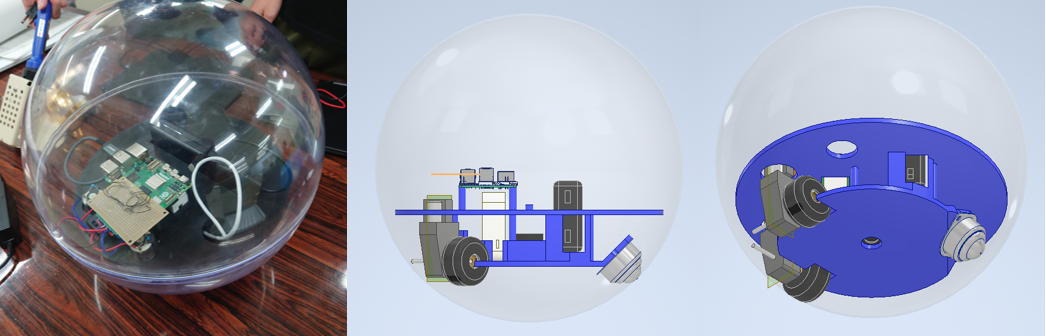
\includegraphics[width=1\hsize]{line-tracer/fig/image1.png}
  \caption{ライントレーサの外観}
  \label{fig:image1}
\end{figure}

\begin{figure}[h]
  \centering
  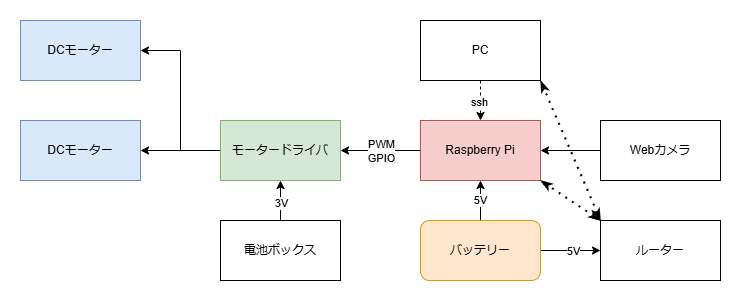
\includegraphics[width=1\hsize]{line-tracer/fig/image2.png}
  \caption{回路系システム}
  \label{fig:image2}
\end{figure}

\section{シミュレーション環境の作成}

\subsection{ランダムコース生成}
ライントレース用のランダムなコース生成は、エージェントの汎化性能を高めるために重要です。単一のコースで学習を行うとエージェントはそのコースに特化してしまい、たとえ同じコースだとしても実世界とシミュレーションのギャップに耐えられなくなってしまいます。そこで、事前に複数のランダムなコースで学習することで、様々な状況に対応できるエージェントを育成します。

コースの生成手順としては、まず領域を4×4のグリッドに分割し、幅優先探索アルゴリズムでスタート地点からゴール地点までの経路を生成します。その後、マスの境界のランダムな位置に線を通すポイントを定め、OpenCVの関数を用いて黒線を描画することでコースを完成させます。その様子を図\ref{fig:image3}に示しています。

\begin{figure}[h]
  \centering
  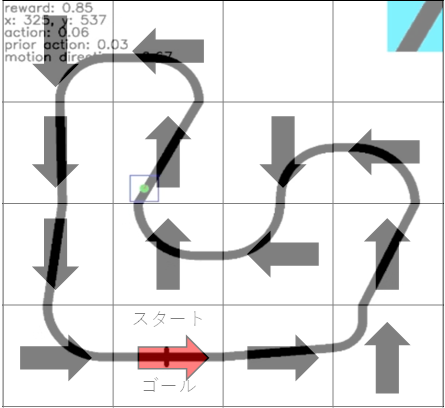
\includegraphics[width=0.7\hsize]{line-tracer/fig/image3.png}
  \caption{コース生成のイメージ}
  \label{fig:image3}
\end{figure}

\subsection{アクションの適用}
エージェントから出力されたアクションは、仮想的なライントレーサの移動方向に変換されます。初期モデルでは、アクションを2次元ベクトルで表現していましたが、コースの途中で停止したり、逆走する等の問題があり、最終的には速度を固定し自由度を削減することで、1次元のスカラーで移動方向を表現する方法を採用しました。

具体的には、図\ref{fig:image4}のように、アクション\textit{action}と概念的な進行方向\textit{action\_average}を用いて、移動方向$\theta$を計算します。なお、\textit{action\_limit}は進行方向に対して、移動方向がどれだけ逸脱できるかを制御するパラメータです。
\[
\theta = (\text{action\_average} + \text{action} \times \text{action\_limit}) \times \pi
\]
これにより、基準方向と移動方向が分離され、エージェントの学習効率が向上するとともに、前述の問題を解決することができました。
\begin{figure}[h]
  \centering
  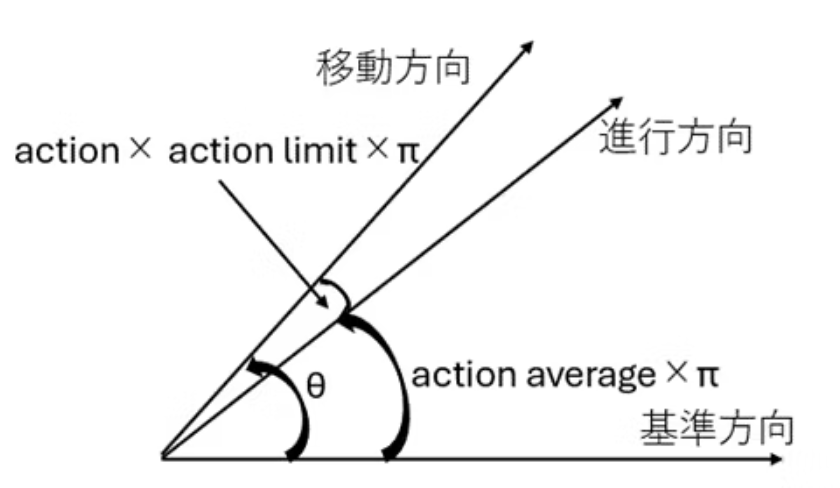
\includegraphics[width=0.7\hsize]{line-tracer/fig/image4.png}
  \caption{移動方向の計算}
  \label{fig:image4}
\end{figure}

\subsection{観測の作成}
本シミュレータでは、エージェントが観測する情報として、ライントレーサ周辺のコースを切り取った64×64のグレースケール画像、進行方向を示すスカラー値、前回のアクションを示すスカラー値の3種類を使用しています。

ただし、Gymの仕様上スカラー値も一度画像に変換し3チャンネルの画像としたうえで、エージェント側に渡しています。

\subsection{報酬関数}
報酬関数は、エージェントの行動を適切に誘導するために設計されます。今回の報酬は2つの要素から構成されています。1つ目は、前回のアクション\textit{previous\_action}とのL1誤差に基づく報酬で、アクションの振動を抑制するために設けられています。2つ目は、観測画像の中心\textit{image\_center}と、黒ピクセル(ライン)の平均座標\textit{black\_center}との距離に基づく報酬で、ロボットをライン上に維持することを目的としています。

\[
\text{reward} = 1 - \frac{| \text{previous\_action} - \text{action} |}{2} - \frac{\| \text{black\_center} - \text{image\_center} \|}{\| \text{image\_center} \|}
\]
これにより、エージェントはライン上をスムーズに移動し続けるように学習します。

\section{エージェントについて}

\subsection{活性化関数と最適化手法の変更}
今回エージェントとして採用したDrQ-v2\cite{yarats2021masteringvisualcontinuouscontrol}は、Metaが開発したQ学習ベースの強化学習アルゴリズムであり、画像を観測として連続値制御が可能な点や処理が軽量である点が特徴です。しかし、2021年の発表以降の技術進歩を踏まえ、今回の実装では活性化関数と最適化手法を変更しました。

まず、DrQ-v2では全ての活性化関数がReLUでしたが、現在はGELUやSiLUが主流です。そこで、画像処理に関わるエンコーダ部分の活性化関数をSiLUに、その他の部分はGELUに変更しました。また、最適化手法もAdamからWeight Decayを導入したAdamWに変更し、パフォーマンスと安定性の向上を図りました。

\subsection{画像とスカラーの同時入力への対応}
DrQ-v2は画像入力を前提としていますが、今回のタスクでは環境から取得した3チャンネルの画像のうち2チャンネルはスカラー情報に過ぎません。これをそのまま画像として処理するのは非効率であるため、エンコーダ部分を改良し、スカラー情報を適切に処理できるようにしました。

具体的には、画像データの内スカラーの情報しか持たない2チャンネルはスカラー値として、CNNには通さずそのまま画像の潜在表現に結合しました。この変更によって、より効率的な学習が可能となりました。

\subsection{パラメータ数の削減}
DrQ-v2の元々のパラメータ設定は複雑なタスクを想定していたため、今回のライントレースタスクに対しては過剰でした。そのため、エンコーダやアクタークリティックのパラメータを削減し、重みのファイルサイズを75158kBから3278kBへと削減しました。

結果として、図\ref{fig:image5}に示すように、若干の劣化が見られるもののモデルは十分な性能を維持しており、Raspberry Pi 5上での制御周期を1Hzから3Hzまで向上させることができました。
\begin{figure}[h]
  \centering
  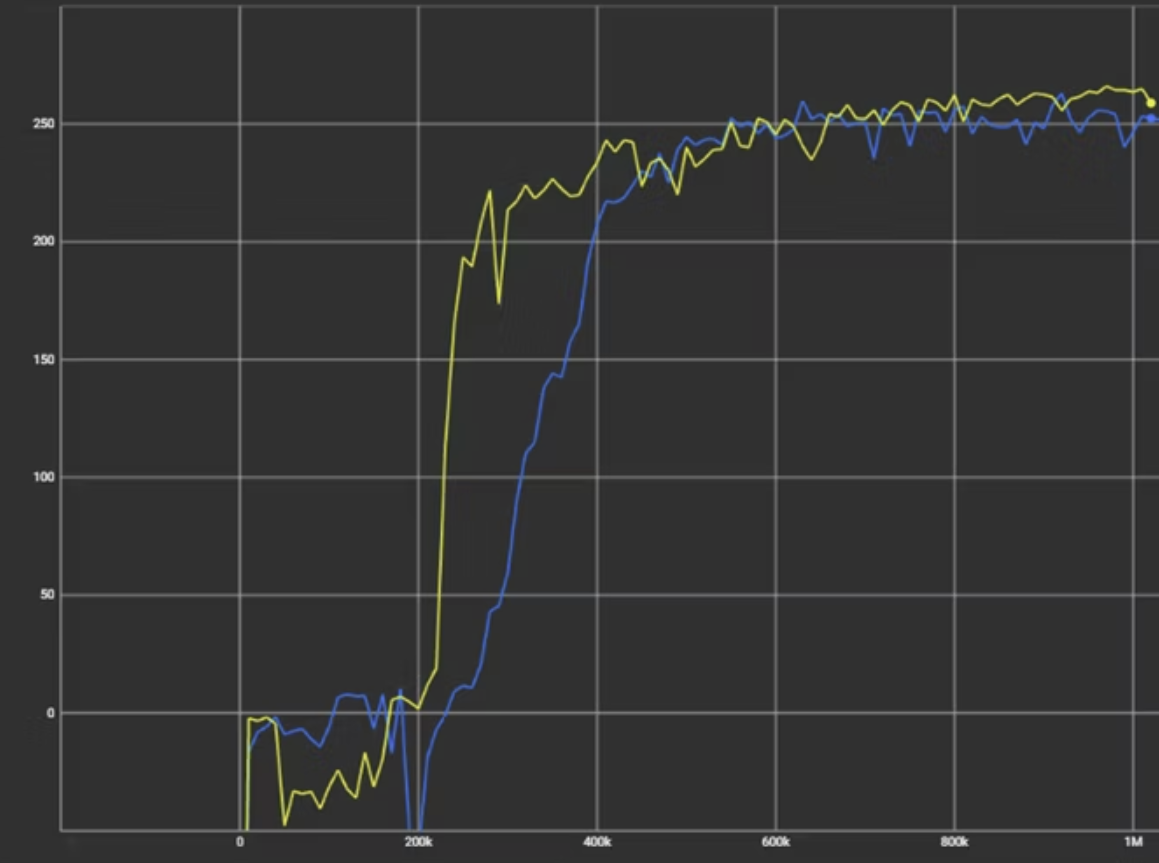
\includegraphics[width=0.7\hsize]{line-tracer/fig/image5.png}
  \caption{報酬の推移(黄色: 変更前のモデル, 青: 変更後のモデル)}
  \label{fig:image5}
\end{figure}

\section{Sim2Real}

\subsection{モータの制御}
シミュレータ上でトレーニングしたモデルを現実世界に持ってくるにあたっては、その差異をどのように減らすのかであったり、埋め合わせるのかということが重要になります。そのため今回のライントレーサは、できるだけシミュレータ上でエージェントの汎化性能を高めたうえで、現実世界の観測をシミュレータの観測に近づけるという方針で実装しました。

強化学習モデルから出力されたアクションは、前述の方法で移動方向$\theta$に変換されます。この移動方向を基に、2つのモータの回転方向とduty(出力比率)を計算し、モータードライバの制御テーブルに従ってGPIOを制御します。GPIOの制御にはRaspberry Pi用のライブラリである\texttt{gpiozero}を使用しています。

\subsection{観測の作成}
次に観測データの作成について述べます。処理の流れとしては、まずWebカメラから取得した1920×1080×3のRGB画像を正方形にトリミングして1080×1080×3にした後、64×64×3に圧縮しています。

次に、圧縮したRGB画像を64×64×1のグレースケール画像に変換し、その画像のピクセルの値の平均$\mu$を求めています。その後、求めた平均値から動的に閾値を計算して、グレースケール画像を二値化し観測としています。
\[
\text{threshold} = \mu \times \text{thresh}
\]
\[
I_{\text{binary}}(x, y) =
\begin{cases}
255 & \text{if } I(x, y) \geq \text{threshold} \\
0 & \text{if } I(x, y) < \text{threshold}
\end{cases}
\]
こうすることで、周辺環境が多少変化したとしても自動的に閾値を調整して、安定的にラインを検出できるようになります。

\section{まとめ}
以下のURLから実機を動作させた時の映像を見る事ができます。

\url{https://youtu.be/tTh6BYUjfMs?si=XSdIw1bt-LwlgnkB}
\begin{figure}[h]
  
\includegraphics[width=0.4\hsize]{line-tracer/fig/QR.png}
\end{figure}

この章では強化学習によって動作するライントレーサについて、全体的なシステム構成や実装方法を説明してきました。

今回、私がライントレーサを製作した目的の一つは、強化学習を実世界のロボットに応用することは可能なのか、また、その過程でどのような困難があるのかを検証するためでした。その結果、シミュレーションと現実のギャップや、処理速度の問題など、普段は意識しないような難しい課題が存在することが分かりました。一方で、それらの課題を解決することができれば、現実世界でも強化学習エージェントを動作させることができました。

現在、ロボティクス領域において、今回紹介した強化学習をはじめとして様々な機械学習技術の応用が行われています。今後も、機械学習とロボティクスという二つの分野が相互に影響を及ぼし、発展していく事を願っています。

ソースコードは\url{https://github.com/Azuma413/rl_linetrace}にて公開しています。


\chapter{目線で操るマウスカーソル}\label{chap:eye-track-cursor}
\section{視線追跡モデルを開発した理由}
近年、AI技術が急速に進化し、画像から様々な情報を取得することが可能になりました。たとえば、物体検出の分野では、Yoloなどの様々なモデルによって、カメラ画像から人や物体の位置をすばやく検出できるようになっています。こうした技術を利用し、視線の位置を特定することができれば、視線を利用した新しい操作インターフェースを提供できるのではないかと考えました。

本プロジェクトの目的は、カメラで取得した視線情報をもとに画面上のカーソルを操作するシステムを開発し、ユーザーが手を使わずに目線のみで操作できる新しいインターフェース体験を提供することです。

\section{全体像}
まず初めに、今回開発した「視線で操作するマウスカーソル」のアプリの全体像について説明していきます。

このアプリでは以下の流れによってユーザーの見ている場所にマウスカーソルを動かします。\\
$\blacksquare$\textbf{マウスカーソルを見ている場所に動かす流れ}
\begin{enumerate}
    \item 4隅を見た時のユーザーの顔画像Tを、PCに内蔵されてあるカメラから取得
    \item TからモデルがPC上で見ている座標を予測し、取得した座標を基に射影変換行列Wを作成
    \item 一定間隔でカメラから顔画像を取得し、顔画像からモデルが予測した座標とWを元に、PC上で見ている座標を予測
    \item 3で予測した座標にマウスカーソルを動かす
    \item 3~4を繰り返し、リアルタイムで見ている場所にマウスカーソルを動かし続ける
\end{enumerate}
射影変換行列Wは「Tから予測した座標を元にモデルが予測したPCの4隅の座標から作られたPCの概形」を「実際のPCの概形」に変換するための行列です。
ここWを用いた理由は、PC上で見ている座標をモデルが予測しても、モデルが予測した座標の単位と実際のPCにおける座標の単位は異なりうるので合わせる必要があるためです。
また、本モデルによる顔画像からのPC上で見ている座標の予測の流れは以下の通りです。\\
\clearpage
$\blacksquare$\textbf{座標予測の流れ}
\begin{enumerate}
    \item 目の位置を推定
    \item 視線の角度を推定
    \item 1.と2.で取得した「視線の角度・目の位置」をもとに、PC上で見ている箇所を計算
\end{enumerate}
以降では、$\blacksquare$\textbf{モデルの推論の流れ}にて言及した「目の位置の推定」と「視線の角度の推定」を行う手順、そして最終的なアプリによる視線の予測結果について説明していきたいと思います。
\section{目の位置の推定}
このモデルは、顔画像から目の位置をPnP問題として考え、推定するモデルです。PnP問題とは「カメラの情報(実際のカメラの位置・やカメラの焦点距離・歪み係数)」と「画面上の物体ととある座標系$D_{world}$(≠カメラを原点とする座標系$D_{camera}$)における物体の位置の関係性」を元に、実際のカメラの位置と回転方向を求める問題です。
\begin{figure}[!ht]
    \centering
    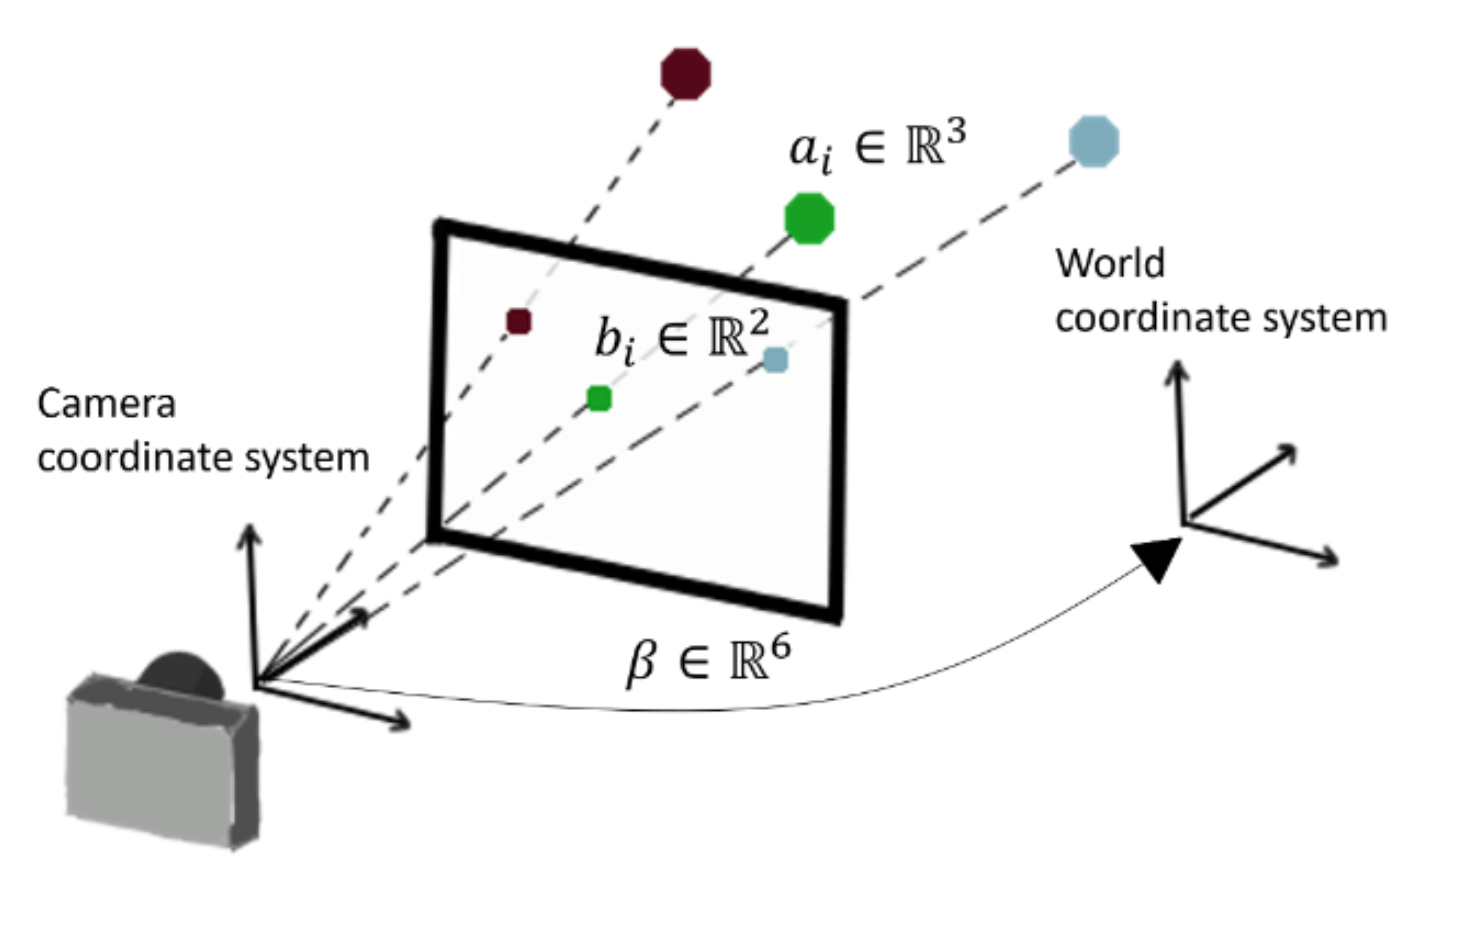
\includegraphics[width=0.7\textwidth]{eye-track-cursor/fig/camera_world_coordinate.png}
    \caption{Camera coordinate system($D_{camera}$)とWorld coordinate system($D_{world}$)の関係性}
    \label{fig:camera_world_coordinate}
\end{figure}
\begin{figure}[!ht]
    \centering
    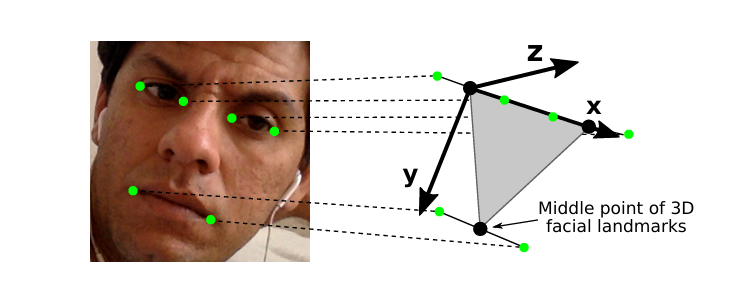
\includegraphics[width=0.7\textwidth]{eye-track-cursor/fig/world_coordinate.png}
    \caption{World coordinate system($D_{world}$)上における顔の特徴点}
    \label{fig:world_coordinate}
\end{figure}
また、顔画像から目の位置を求める流れは以下の通りで、\cite{zhang2017mpiigaze}を元に作成しました。\\
$\blacksquare$\textbf{目の位置を推定する流れ}
\begin{enumerate}
    \item dlibを使用し、画像上における顔の特徴的な部分(目や鼻など)を検出
    \item 「カメラの情報(実際のカメラの位置やカメラの焦点距離・歪み係数)」と「1.で検出した特徴点と$D_{world}$上での一般的な顔における関係性」をもとに、\texttt{cv2.solvepnp}を使用してカメラの$D_{world}$上での位置と向き取得
    \item 「1.で求めた画像上での目の場所」と「2.で求めた$D_{world}$上でのカメラの位置と向きから考えられる$D_{camera}$上での頭の位置と向き」を元に、$D_{camera}$上での目の座標を取得
\end{enumerate}
なお、dlibは顔のランドマーク(鼻の位置や目の位置など)を予測するためのモデルで、今回はERTベースのモデル\cite{valle2018deeply}を使用しております。
\section{視線の角度推定}
次に、視線の角度を推定するモデルの開発を行いました。このモデル開発においては複数の手法を試しましたので、それらを1つづつ説明していきます。

\subsection{視線の角度推定(手法1)}
手法1においては、\cite{zhang2017mpiigaze}にて紹介された視線の角度推定モデルを用い、応用しました。
推定の流れは以下の通りです。\\
$\blacksquare$\textbf{視線の角度を推定する流れ}
\begin{enumerate}
    \item $\blacksquare$\textbf{目の位置を推定する流れ}(1.3章)の2.から、顔の向きRとカメラの位置を取得
    \item \texttt{cv2.warpPerspective}でRとカメラの位置に基づき、$D_{world}$上での目の画像(60×36)を生成
    \item 生成した画像をモデルに入力し、視線角度Sを予測
    \item SとRをもとに、実際のカメラから見た視線情報を算出
\end{enumerate}
また、$\blacksquare$\textbf{視線の角度を推定する流れ}の3.にて言及したモデルの構造は以下の通りです。\\
$\blacksquare$\textbf{モデルの構造}
\begin{itemize}
    \item 1層目:EfficientNet(b0)
    \item 2層目:Conv2d
    \item 3層目:Linear+ReLU+Dropout
    \item 4層目:出力値にRを結合
    \item 5層目:Linear+ReLU+Dropout+Linear
\end{itemize}
論文\cite{zhang2017mpiigaze}では、EfficientNetではなくVGG-16を用いておりました。しかし、VGG-16よりもEfficientNetの方が計算量が小さく、一般的な画像認識タスクにおける精度も上回っていることから、EfficientNetを採用しました。このモデルによって、顔の向き(yaw,pitch)を用いて視線方向を実用可能な時間(0.04秒/枚)で推論できました。\\
また、optimizerとしてAdamを、スケジューラーとしてStepLRを用いました。\\
※1層目のEfficientNetにおける最初の層はconv2d(出力チャンネル数:32・カーネルサイズ:3・ストライド:2)に変更しました。\\
そして、このモデルの学習に使用したデータは以下の通りです。
$\blacksquare$\textbf{学習用データ}
\begin{itemize}
    \item MpiiGaze(片目の画像(60×36)と視線情報・顔の向き情報を含むデータセット)
\end{itemize}
yawとpitchの定義は\ref{fig:yaw_pitch_measurement}に書かれてある通りです。\\
\begin{figure}[!ht]
    \centering
    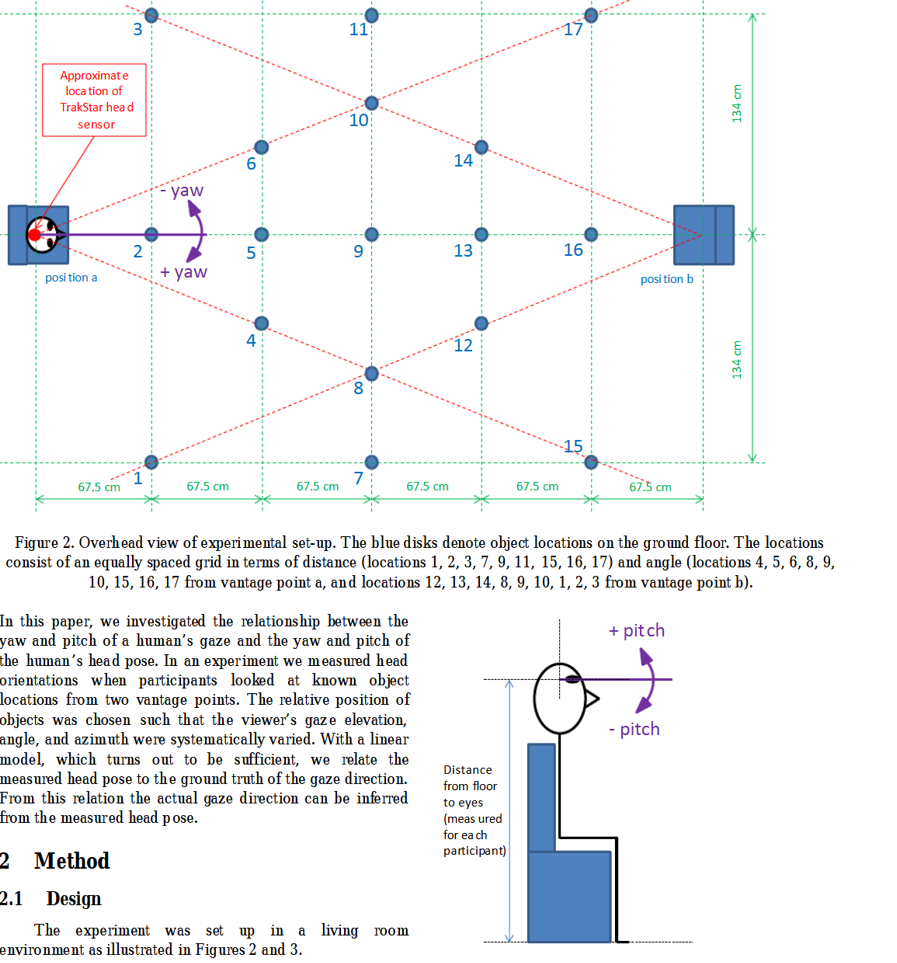
\includegraphics[width=0.7\textwidth]{eye-track-cursor/fig/gaze_definition.png}
    \caption{yawとpitchの定義}
    \label{fig:yaw_pitch_measurement}
\end{figure}
しかし、結果は失敗に終わってしまいました。考えられる要因とその根拠としたことは以下の通りです。\\
$\blacksquare$\textbf{考えられる原因}
\begin{itemize}
    \item 使用したデータの視線角度範囲が狭く、±20°の範囲に限定されていたため
\end{itemize}
$\blacksquare$\textbf{根拠としたこと}
\begin{itemize}
    \item 訓練結果によると学習時のロスは少なく、テスト時においても少なかった
\end{itemize}
\subsection{視線の角度推定(手法2)}
手法2においては、画像から直接視線の角度を推定する外部モデル(AxGazeEstimation)を活用しました。モデルの推論の流れや実験結果などは以下の通りです。\\
$\blacksquare$\textbf{視線推定モデル(AxGazeEstimation)による推論の流れ}
\begin{enumerate}
    \item BlazeFace\cite{bazarevsky2019blazeface}によって顔とその特徴点(目や鼻など)を検出
    \item 1.にて検出した顔とその特徴点を用いて、ResNetの縮小版(stage3モデル)によって視線角度を推定
\end{enumerate}

$\blacksquare$\textbf{結果}
\begin{itemize}
    \item 視線角度の推定に成功しました。(\ref{fig:gaze_direction_estimation_success})
\end{itemize}

\begin{figure}[!ht]
    \centering
    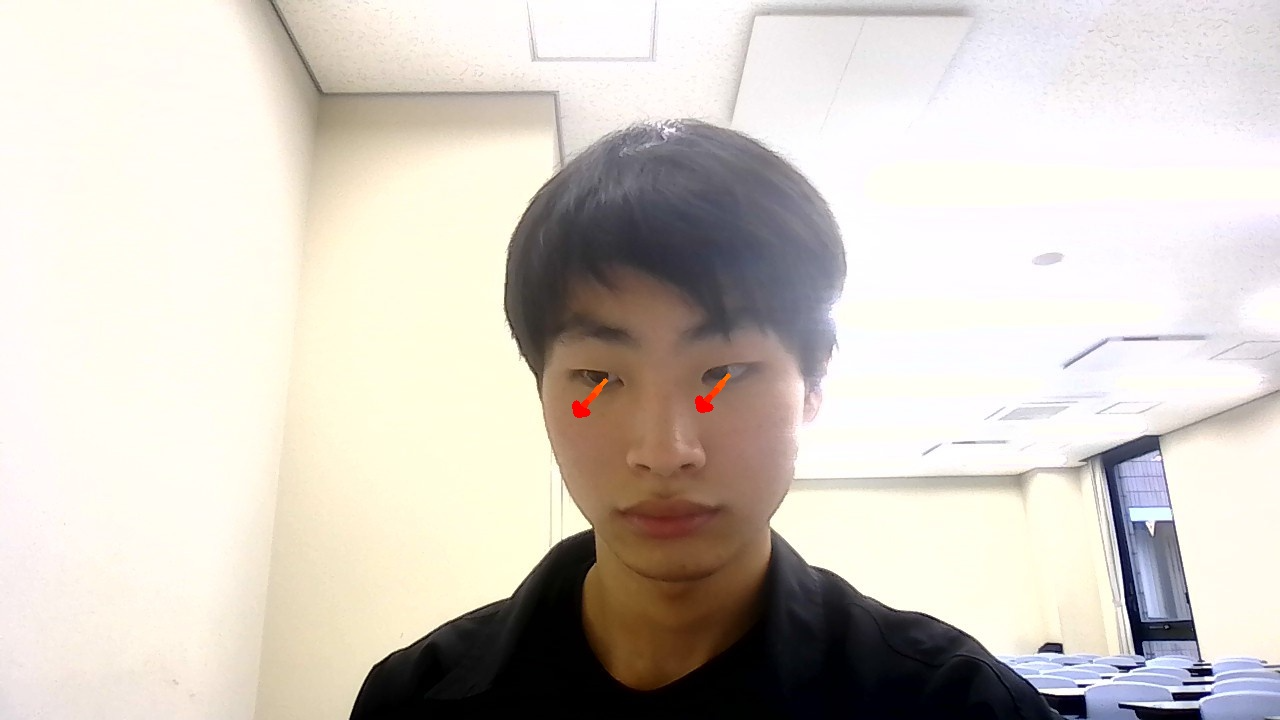
\includegraphics[width=0.7\textwidth]{eye-track-cursor/fig/gaze_direction_result.png}
    \caption{視線角度推定の結果}
    \label{fig:gaze_direction_estimation_success}
\end{figure}
この結果から、視線の角度推定では手法2を採用することにいたしました。
\section{最終結果}
1.2章にて言及した手順を用い、1.3~1.4章にて言及したモデルを用いることで、見ている場所をリアルタイムで推測できるモデルを開発できました。そして、\ref{fig:gaze_estimation_success}のように視線の位置をとらえることができました。\\

\begin{figure}[!ht]
    \centering
    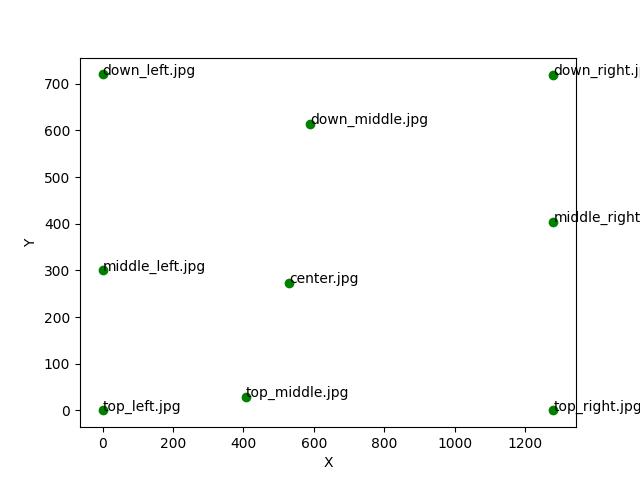
\includegraphics[width=0.7\textwidth]{eye-track-cursor/fig/gaze_at_result.png}
    \caption{視線角度推定の最終結果}
    \label{fig:gaze_estimation_success}
\end{figure}
※画面上のx座標・y座標におけるPCとの関係性は\ref{fig:definition_coordinates}です。
\begin{figure}[!ht]
    \centering
    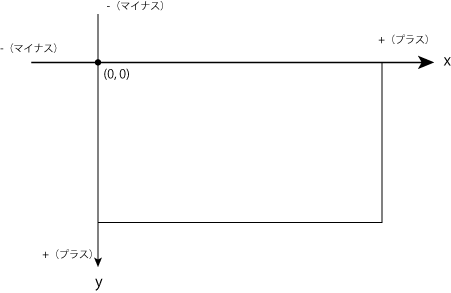
\includegraphics[width=0.7\textwidth]{eye-track-cursor/fig/pc_definition.png}
    \caption{PC上のスクリーン座標系 (x: 0~1280, y: 0~720)}
    \label{fig:definition_coordinates}
\end{figure}
\section{さいごに}
最終的にモデルを作成できましたが、第1.4.1章で考案した手法ではうまくいきませんでした。しかし、データに問題があるのかもしれないと考えられます。このことから、モデルだけでなく、データもきちんと選定する重要性があることが分かりました。\\
他にも様々なyaw,pitchに関する学習モデルが存在し、yaw,pitchの範囲が広い学習データもありましたが、どのデータもデータサイズが大きく、ダウンロードしにくい状況でした。そのため、今後はモデルについて考察するだけでなく、データ選定の手法についても学ぶ必要があることが分かりました。\\
また、今後はデータのyawやpitchの範囲が-20°~20°と狭いことが影響している可能性があるため、yawやpitchが±20°に近い角度のデータの比重を高め、モデルが広範囲の視線角度に対しても正確に推定できるようにして実験したいです。\\
\begin{figure}[!ht]
    \centering
    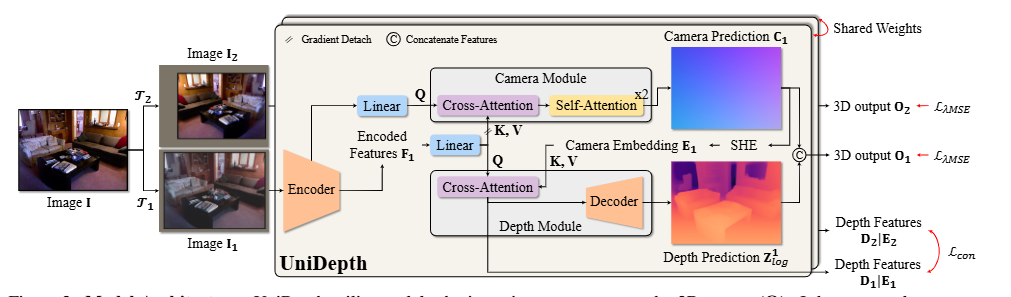
\includegraphics[width=0.7\textwidth]{eye-track-cursor/fig/UniDepth.png}
    \caption{UniDepthの構造}
    \label{fig:UniDepth}
\end{figure}
また、深度推定においてUniDepth(\ref{fig:UniDepth})などの様々な深度推定モデルがございました。そのため、今後はそういったモデルによって目とカメラの距離を求め、それを元に目とカメラとの位置関係を求めるようにしていきたいです。


\chapter{KaiRAくんを動かそう}\label{chap:moving-kaira-kun}
\section{はじめに}

当サークルのマスコットキャラクターであるKaiRA君を動かして愛でてみたい、というのがこのプロジェクトを製作した動機です。当プロジェクトでは、ユーザーが自然言語による命令を入力すると、KaiRA君がそれに従って動いてくれます。命令と動きによる応答の関係を通じて、時には命令にうまく従ってくれないことも含め、KaiRA君との不思議な交流が楽しめます。

\begin{figure}[htbp]
    \centering
    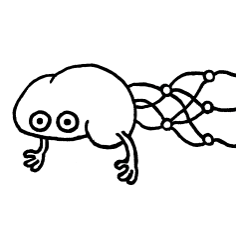
\includegraphics[width=0.5\textwidth]{moving-kaira-kun/fig/kaira_kun.png}
    \caption{当プロジェクトで使用したKaiRA君のイラスト}
    \label{fig:kaira_kun}
\end{figure}

\section{モーションの生成}

KaiRA君のモーションを自然言語から生成するために、当プロジェクトではHuman Motion Diffusion Model\cite{tevet2022humanmotiondiffusionmodel}を用いています。テキストからモーションを生成するモデルはこれ以外にも、MotionGPT\cite{jiang2023motiongpthumanmotionforeign}等が挙げられます。しかし、生成されるモーションの質に大きな差が見られなかったので、生成速度の観点からこの手法を選択しました。Human Motion Diffusion Modelは、ノイズを50ステップという少ないステップ数で取り除いても十分な質のモーションを生成できます。

Human Motion Diffusion Modelはその名の通り、基本的な生成の仕組みは拡散モデルに基づいています。Transformerのエンコーダ部分を用いて、各時刻における関節の位置や回転が予測されています。ただし、学習に用いられる損失関数には工夫が施されていて、通常の拡散モデルによる手法のものとは異なります。通常はある時刻で与えたノイズと、それを予測したノイズとの間で損失を取りますが、この手法ではノイズが加えられる前のものと、ある時刻でノイズが除去された後のものとの間で損失を取っています。これに、各関節の位置や速度の予測と正解の差を考慮した損失を組み合わせたものを用いて、学習を行っています。

\begin{figure}[htbp]
    \centering
    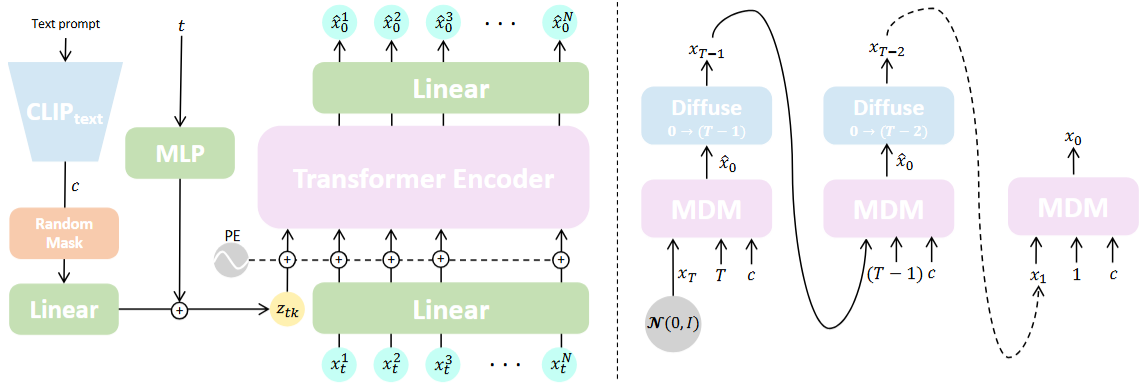
\includegraphics[width=0.8\textwidth]{moving-kaira-kun/fig/hdm_overview.png}
    \caption{Human Motion Diffusion Modelの全体像}
    \label{fig:hdm_overview}
\end{figure}

Human Motion Diffusion Modelで生成されたモーションは、NumPy配列として出力されます。当プロジェクトでは、出力されたNumPy配列をBVHファイルに変換したものをAnimated Drawingsに入力しています。

\section{アニメーションの生成}

生成されたモーションに従ってKaiRA君を動かすために、当プロジェクトではAnimated Drawings\cite{smith2023methodanimatingchildrensdrawings}を用いています。実のところ、当初は2Dのアニメーションではなく、KaiRA君の画像から生成した3Dモデルを用いるつもりでした。しかし、LRM\cite{hong2024lrmlargereconstructionmodel}やDreamGaussian\cite{tang2024dreamgaussiangenerativegaussiansplatting}等の手法を試したものの、平面的な1枚のイラストを3Dにうまく変換することはできませんでした。そのような経緯で、3Dモデルを生成することは一旦諦め、KaiRA君を2Dのイラストのまま動かすことにしました。

Animated Drawingsは、キャラクターの関節の位置を1枚の画像から推定し、それを基づいてアニメーションを生成することが可能です。しかし、学習に用いられたイラストは人の形をしたものが多いため、KaiRA君に対して自動で関節を割り当ててもうまく機能しません。また、KaiRA君は人間のような下半身を持たないため、生成された人間のモーションをそのまま適用すると、胴体がねじれる等の不都合が生じます。そこで当プロジェクトでは下図のように、腕の動きを反映させることを重視し、下半身の関節については画像の下端に配置することで、その影響をなるべく排除しています。

\begin{figure}[htbp]
    \centering
    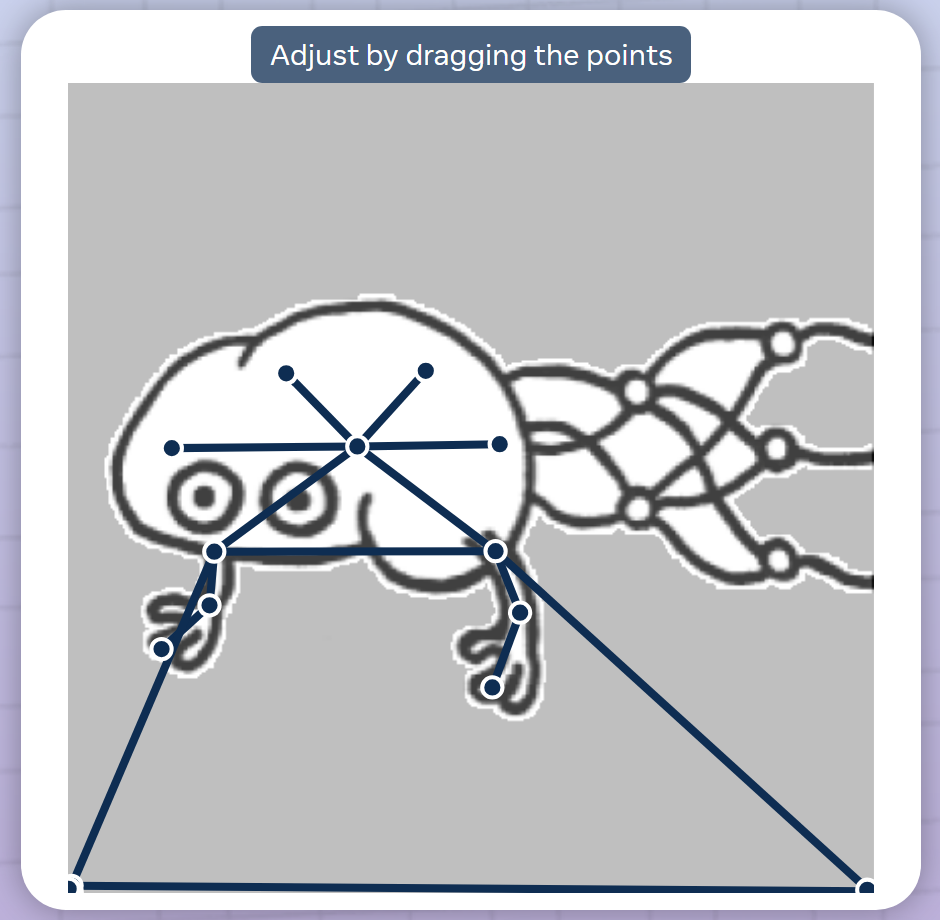
\includegraphics[width=0.5\textwidth]{moving-kaira-kun/fig/kaira_kun_animated_drawings.png}
    \caption{KaiRA君の関節の配置の設定}
    \label{fig:kaira_kun_animated}
\end{figure}

Animated DrawingsはBVHファイルにより、アニメーションの動きを指定することができます。このとき入力されるモーションは3Dですが、これを平面に投影することでキャラクターの関節と対応させています。ただし、BVHファイルの関節と、キャラクターの関節との対応関係は手動で設定する必要があります。

\begin{figure}[htbp]
    \centering
    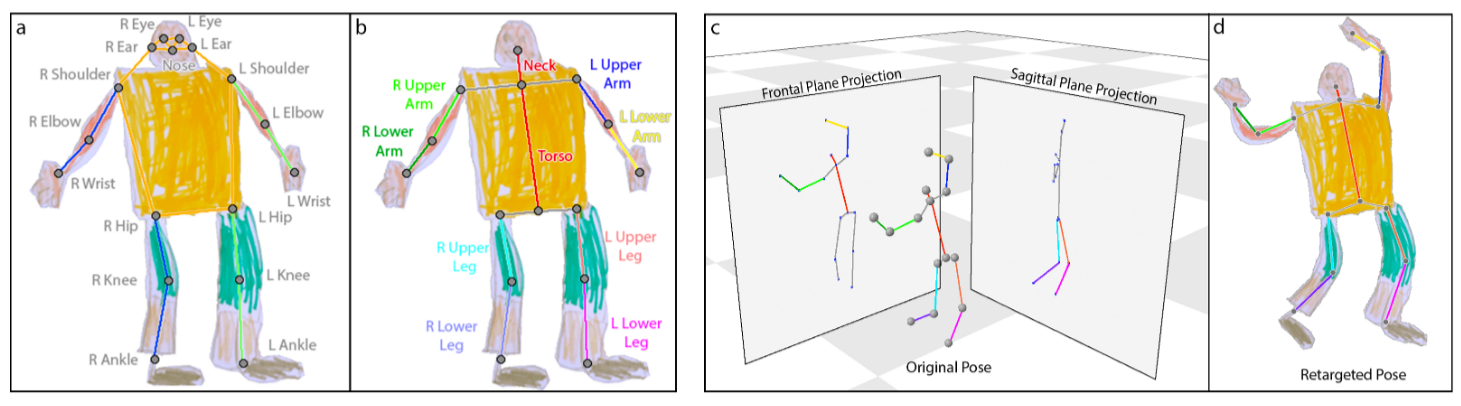
\includegraphics[width=0.8\textwidth]{moving-kaira-kun/fig/animated_drawings.png}
    \caption{Animated Drawingsの全体像}
    \label{fig:animated_drawings}
\end{figure}

Animated Drawingsの手法の詳細には立ち入りませんが、これをHuman Motion Diffusion Modelと組み合わせることで、自然言語の命令によりKaiRA君をアニメーションで動かすことが可能になります。

\section{おわりに}

現在のAIはすでに高度な言語処理能力を持つようになりましたが、現実の人間による言語活動は純粋な言語でのみ構成されるものではなく、身体的な要素が多大に含まれています。その意味では、言語と身体を繋ぐ道具として、テキストからモーションを生成する手法は想像以上に重要かもしれません。当プロジェクトでは人間が入力したテキストを用いてモーションを生成していますが、AIが自ら適切なモーションを選択し生成できるようになれば、人間とAIのコミュニケーションはより豊かなものになり得ると思います。


\chapter{最強じゃんけんAI}\label{chap:no-lose-janken}
\section{概要}
この「じゃんけんAI」では、リアルタイムの映像から手の形を推測し、各時刻ごとに手の動きを予測しています。じゃんけんの大規模な動画データを用意するのが難しく、独自の小規模なデータで学習を行うために、学習済みの骨格推定モデルを用いて映像から手の位置や形を骨格データとして抽出し、骨格データからじゃんけんの手を推測する方法を取りました。この骨格の時系列データをもとに、次の瞬間の手の形状を予測するためにリカレントニューラルネットワーク(RNN)を活用しました。RNNの時系列予測の強みを活かし、じゃんけんの手の変化に応用することで、手を出し終わる前に予測を行い、後出しではなく自然な流れでじゃんけんができるよう工夫しています。

\section{骨格推定モデル}
骨格推定とは、人間の関節や目、鼻などの特徴点(ランドマーク)の位置を推定する技術であり、深度センサーや慣性センサーなどの高度な機器を用いた高精度な3次元推定から、通常のカメラを用いた2次元画像からの推定まで、幅広い手法が存在します。代表的な骨格推定モデルには、カーネギーメロン大学の「OpenPose」やGoogleの「MediaPipe」、および「PoseNet」などがあります。今回のじゃんけんAIでは、リアルタイムに手の動きを認識する必要があるため、「MediaPipe」 を採用しました。MediaPipeは、他のライブラリと比較して高速なリアルタイム処理に優れており、手のみの骨格推定を行うことが出来ます。手の骨格推定では、手の写った画像から21個の関節位置を検出し、深度推定を用いて3次元座標に推論することができます。
\begin{figure}[h]
  \centering
  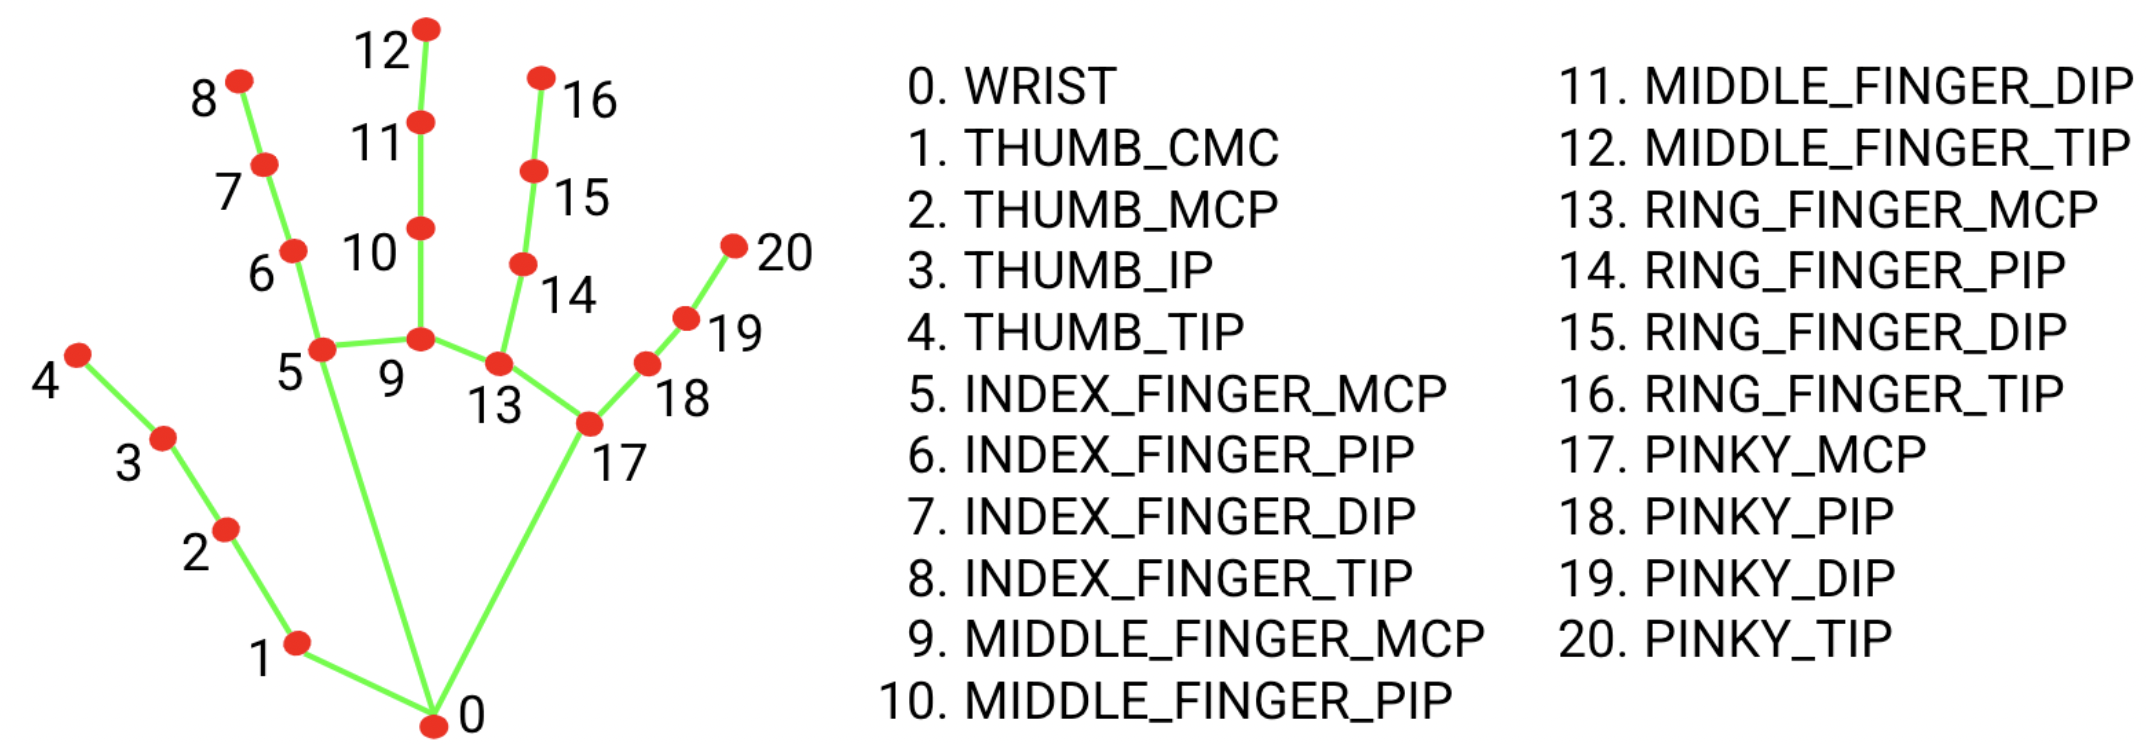
\includegraphics[width=10cm]{no-lose-janken/fig/hand-landmarks.png}
  \caption{mediapipeの検出する手の骨格}
  \label{fig:hand_landmark}
\end{figure}

\section{実験}
\subsection{データ}
学習データとして、独自に用意した246本のじゃんけん動画を使用しました。データ作成時には、多様性を確保するために、さまざまな手の握り方や角度を含めるよう意識しました。データ数が少ないため、手の平行移動を利用したデータ拡張を行ったところ、精度が大幅に向上しました。また、右手のデータのみを用いていたため、リアルタイム推論時に左手の認識がやや不安定になるという問題がありましたが、左右反転のデータ拡張を加えることで、左手も右手と同等の精度を実現しました。

\subsection{時系列予測}
骨格の時系列データの処理には、RNN・LSTM・GRUを用いて精度と推論時間の比較を行いました。時系列データを扱う強力なモデルとしてTransformerも考慮しましたが、今回は小規模なデータセットによる学習であることから使用しませんでした。

最初は、手を出す2秒前(60フレーム分)のデータで学習を行い、精度は\ref{tb:60frame}のようになりました。手を出す直前での精度はに違いは見られませんでしたが、タイミングが離れるほどRNNの精度が低下し、LSTMとGRUに関しては、1秒前まではほぼ同等の精度となりますが、2秒前になるとLSTMの方が少し精度が良くなります。しかし、学習時の2秒前の精度の高さに反し、リアルタイムで推論を行う際には、手を出す前はほとんどが「グー」となり、さらに推論が不安定になってしまいました。

手の形が変化しだすのが、手を出す約0.15秒前であることから、学習データとして手を出す瞬間の前後約0.2秒の15フレームを学習させることにしました。この15フレームでの学習では、\ref{tb:15frame}のようにRNN,LSTM,GRU全てで全時刻精度1となり、リアルタイム推論でも安定して精度よく推論できるようになりました。

\begin{table}[h]
       \hspace{0.1\textwidth}%
       \begin{subtable}{0.3\textwidth}
           \centering
           \begin{tabular}{l||c|c|r}
              & RNN & LSTM & GRU \\ \hline\hline
              2秒前 & 0.596 & 0.914 & 0.876 \\ \hline
               & 0.617 & 0.965 & 0.943 \\ \hline
               \vdots & \vdots & \vdots & \vdots \\ \hline
               & 0.684 & 0.979 & 0.980 \\ \hline
              1秒前 & 0.676 & 0.979 & 0.980 \\ \hline
               & 0.664 & 0.979 & 0.980 \\ \hline
               \vdots & \vdots & \vdots & \vdots \\ \hline
               & 0.984 & 0.985 & 0.985 \\ \hline
              ポン & 0.984 & 0.985 & 0.985 \\ \hline
           \end{tabular}
           \caption{60フレーム学習の精度比較}
           \label{tb:60frame}
       \end{subtable}%
       \hspace{0.1\textwidth}%
       \begin{subtable}{0.3\textwidth}
           \centering
           \begin{tabular}{l||c|c|r}
              & RNN & LSTM & GRU \\ \hline\hline
              -7フレーム & 1.00 & 1.00 & 1.00 \\ \hline
               & 1.00 & 1.00 & 1.00 \\ \hline
               \vdots & \vdots & \vdots & \vdots \\ \hline
               & 1.00 & 1.00 & 1.00 \\ \hline
              ポン & 1.00 & 1.00 & 1.00 \\ \hline
               & 1.00 & 1.00 & 1.00 \\ \hline
               \vdots & \vdots & \vdots & \vdots \\ \hline
               & 1.00 & 1.00 & 1.00 \\ \hline
               +7フレーム& 1.00 & 1.00 & 1.00 \\ \hline
           \end{tabular}
           \caption{15フレーム学習の精度比較}
           \label{tb:15frame}
       \end{subtable}%
   \end{table}

\subsection{推論速度}
推論速度としては全データを推論するのにかかる時間は図のようになり、全モデルでGPUよりもCPUでの推論が早く、CPUでの推論速度はRNN>GRU>LSTMとなりました。15フレームの学習では精度が変わらないので、cpuでの推論速度が一番速いRNNを採用しました。
\begin{table}[h]
           \centering
           \begin{tabular}{l||c|c|c|r}
              &RNN&LSTM&GRU\\ \hline\hline
              GPU & 241 & 202 & 243\\ \hline
              CPU & 74 & 135 & 114 \\ \hline
           \end{tabular}
           \caption{GRU}
\end{table}

\section{結論}
今回のじゃんけんAIでは、時系列予測を活用して後出しではない自然な動作を目指し、最終的に手を出し終わる前に正しい手を予測するモデルを開発することが出来ました。しかし、実際にじゃんけんをする際には、画面とのタイミングを人間側で合わせるのが難しく、モデル以外の部分に課題が残ります。今後は、人とAIのタイミングをさらに自然にする工夫を加え、よりスムーズなじゃんけんAIを目指していきたいと思います。


\chapter{京大シラバス検索RAGシステム - システム概要編}\label{chap:syllabus-rag-overview}
\section{京大シラバスRAGシステムの基本情報}
\subsection{シラバスとRAGシステム}
シラバスとは、京都大学情報教務システムKULASISが公開している京都大学の科目の情報が載っているページである。これは京都大学の学生・職員でなくとも閲覧することができる。シラバス検索というページから、知りたい科目の条件(学部、学科、曜時限等)で検索をして、各科目のページに飛ぶことができる。各科目のページには以下のような項目がある。括弧の中の項目は一部の科目にある。\\

\begin{itemize}
  \item 科目ナンバリング、科目名、英訳
  \item 所属部局・職名・氏名
  \item 使用言語、単位数、授業形態、開講年度・開講期、配当学年、対象学生、曜時限、(時間数)、(キーワード)
  \item 授業の概要・目的、到達目標、授業計画と内容、(題目)
  \item 履修要件、成績評価の方法・観点、教科書、参考書等、授業外学修、(関連URL)、(実務経験のある教員による授業)
\end{itemize}

RAG(Retrieval-Augmented Generation)とは、LLM(大規模言語モデル)の文章生成に外部データの検索機能を組み合わせる手法である。似た手法にファインチューニングがあるが、これは事前学習されたLLMをさらに外部データで学習させる手法である。今回は外部データを京大シラバスとして、RAGシステムを実装した。また、1つの検索対象のテキストの集まりを\emph{チャンク}と呼ぶ。\\

今回の実装では、\emph{データの埋め込み}(文章をベクトル化すること)の計算が多く、前処理を変更するたびに埋め込みをすると時間がかかるので、大学院の専門科目(約10000科目)を除いた全学共通科目と学部の専門科目(約8000科目)だけを利用した。さらに、この中で医学部医学科だけがシラバスがPDFで個別の処理が必要なので、医学部医学科の科目も除外した。最終的に外部データとしたのは、全学共通科目と医学部医学科以外の学部の専門科目となった。\\

\subsection{実装の優先事項と概要}
今回の実装をするに当たって、自分が最も重要視したことが実用性である。RAGシステムの基本的な流れは、ChatGPTなどと同様に質問を入力して、質問のテキストと類似度が高い外部データのテキストを抽出し、質問と抽出したデータを入力としてLLMで回答を生成する。今回の実装したRAGシステムは、京都大学の学生の要求に対応した科目の検索ができるようになることを想定している。従って、質問と類似度が高い外部データのテキストを抽出する前に、外部データの\emph{絞り込み}が必要だと考えた。つまり、シラバス検索ページのような科目の条件(学部、学科、曜時限等)で絞り込みをする機能をRAGシステムに組み込む形で実装をすることに決めた。\\

実装で使用したプログラミング言語はpythonで、主に使用したライブラリは、LLMの機能拡張をするためのLangchainから外部データの埋め込みを扱えるFAISSと、前処理をする際にHTMLからテキストを抽出するためのBeautifulsoupと、python上で簡易的にアプリ化するstreamlitである。LLMのモデルは無料で公開されているGoogleが開発した生成AIモデルであるGemini-pro、埋め込みのモデルはHuggingFaceEmbeddingsの多言語に対応しているintfloat/multilingual-e5-baseを使用した。\\

\section{絞り込み}
\subsection{KULASISの絞り込みのための検索項目}
科目の条件で絞り込みを行うときに参考にするのは、もちろんKULASISのシラバス検索だが、これには京都大学の学生・職員でなくとも利用できる\emph{全科目のあるシラバス検索}と、京都大学の学生・職員がログインして利用できる\emph{全学共通科目だけのシラバス検索}と、スマートフォンでの\emph{KULASISアプリで利用できるシラバス検索}が存在し、少し検索項目に違いがあることが分かった。それぞれの検索項目を表にすると表1のようになった。\\

\begin{table}[h]
\centering
\caption{シラバス検索の検索項目}
\begin{tabular}{cccc}\hline
 & 全科目のシラバス & 全学共通科目のシラバス & アプリのシラバス\\ \hline
学部/大学院& 〇 & / & 〇\\
課程& × & 〇 & 〇\\
学科& 〇 & / & 〇\\
群& 〇 & 〇 & 〇\\
旧群& ×& × & 〇\\
開講期& 〇 & 〇 & 〇\\
曜時限& 〇 & 〇 & 〇\\
授業形態& 〇 & 〇 & 〇\\
E科目& × & 〇 & 〇\\
使用言語& 〇 & 〇 & 〇\\
対象学生& × & 〇 & 〇\\
レベル& 〇 & 〇 & 〇\\
学問分野& 〇 & 〇 & 〇\\
科目名& × & 〇 & 〇\\
キーワード& 〇 & 〇 & 〇\\
教員名& 〇 & 〇 & 〇\\
実務経験科目& × & 〇 & 〇\\ \hline
\end{tabular}
\end{table}

説明が必要だと感じた検索項目は以下のようになる。\\

\begin{itemize}
  \item 課程----学部、大学院
  \item 旧群----A群、B群、C群、D群(平成25から27年の入学者向け)
  \item 開講期----前期、後期、前期集中、後期集中など
  \item 授業形態----講義、演習、実験など
  \item E科目----E1、E2、E3
  \item 対象学生----全学向、文系向、理系向、留学生
  \item レベル----導入的な内容、基礎的な内容、発展的な内容、卒業論文・卒業研究関連など
  \item 学問分野----情報学基礎、地球環境学、哲学、言語学など
  \item 科目名----科目名に含まれる文字を入力する
  \item キーワード----シラバスに載っている言葉・文字を入力する
  \item 教員名----担当教員に含まれる文字を入力する
  \item 実務経験科目----実務経験科目の主要な4つ形式の科目とその他の科目
\end{itemize}

シラバス検索から絞り込みに使う検索項目について以下のように整理して考えた。\\

\begin{itemize}
  \item 各科目のシラバスのページ以外にシラバス一覧のページから細かい科目の区分の情報が得られる。
  \begin{itemize}
    \item 全学共通科目の群の中でも、例えば人文社会科目の中に哲学・思想、歴史・文明、地域・文化などのさらなる区分が存在する。これらの区分を\emph{分野}とする。
    \item 学部の中には、工学部のように地球工学科や物理工学科などの学科の区分や、総合人間学部のように人間科学系や国際文明学系などの学科以外の区分が存在する。これらの区分を\emph{学科など}とする。
  \end{itemize}
  \item \emph{レベル}と\emph{学問分野}は各科目のシラバスのページに情報が載っていないので、前処理でこの情報を取り出せず、絞り込みに利用するのは困難である。
  \item \emph{課程}はそもそも今回の実装では大学院の専門科目を除外しているので、絞り込みに利用する価値が低い。
  \item \emph{旧群}は現在適用される人がいないので絞り込みに必要ない。
  \item \emph{科目名}は\emph{キーワード}に包含されることが可能である。
  \item \emph{実務経験科目}は選択肢の文章が長く見栄えが悪い上に、そもそも実務経験科目が少なく絞り込みに利用する価値が低い。
\end{itemize}

以上のことからKULASISのシラバス検索から絞り込みに使う検索項目は、\emph{学部、学科など、群、分野、開講期、曜時限、授業形態、E科目、使用言語、対象学生、キーワード、教員名}とした。\\

\subsection{追加した絞り込みのための検索項目}
今までは、検索項目はシラバスのページから容易に抽出できることが前提だった。しかし、LLMを利用すれば、各科目のシラバスの内容から新たに検索項目を生成できる。どのように検索項目を生成するのかを詳しく説明すると、入力に対する出力が必ずJSONというデータ形式になるモードである\emph{JSONモード}を使用する。検索項目として生成するのは、KULASISの検索項目で抽出が困難だとして断念した\emph{レベル}や\emph{学問}の他に、シラバスの履修要件にある履修していることが望ましいとされた科目や、シラバスの成績評価の方法・観点にある定期試験や平常点などの評価指標の占める成績評価の割合などが考えられる。\\

しかし、検索項目を生成するにはOpenAIへのリクエストが必要であり、Geminiであれば1分間に15リクエスト、1日に約1500リクエストという上限がさだめられている。これでは、約8000個のシラバスのデータから検索項目を生成するには、多くの実行時間や日数が必要となる。これらを削減する手段として以下のようなものがある。\\

\begin{enumerate}
  \item 複数のAPIキーを使用する
  \item 同時に複数の科目のテキストを入力として検索項目を生成する
  \item 同時に複数の種類の検索項目を生成する
\end{enumerate}

今回の実装では、まずは検索項目は有用性の観点から成績の評価指標の割合を追加することにしたが、手法2を試すと複数の科目が、例えば哲学1とその他の哲学1のように科目の内容が被ったときに、出力が1つになって上手く行かなかった。時間の兼ね合いもあり、検索項目は有用性の観点から\emph{成績指標の割合}だけを追加した。

\subsection{絞り込みの方法1 metadatas}
絞り込みの検索候補は決定した。次に絞り込みの方法を説明する。OpenAIの機能拡張するLangchainのFAISSにはmetadatasという機能がある。これは外部データを埋め込みするときに、辞書形式のmetadataをチャンクに一対一対応で登録する。metadataには大きく2つの機能がある。1つ目はフィルタリングで、指定したmetadataのkeyとvalueを持つチャンクのみに類似度検索をできる機能である。2つ目は検索したチャンクにmetadataのkeyを指定することで、metadataのvalueを引き出せる機能である。質問のテキストはquery(int)、外部データはtexts(list)として、metadatasを用いたRAGを実行すると以下のようになる。\\

\begin{lstlisting}[caption=metadatasの例,label=fuga]
metadatas = [{'name':'philosophy',classtype':'lecture','timetable':'Tu2'},
             {'name':'thermodynamics','classtype':'lecture','timetable':'Fr2'},
             {'name':'physics experiment','classtype':'experiment','timetable':'Mo3,Mo4,Tu3,Tu4'}]
store = FAISS.from_texts(texts,embedding,metadatas)
a = store.similarity_search(query,filter={classtype':'lecture','timetable':'Tu2'})
for i in range(len(a)):
    print(a[i].metadata['name'])
\end{lstlisting}

\subsection{絞り込みの方法2 delete}
metadatasの機能は便利だが、metadatasによる絞り込みはmetadataの複数のkeyを指定するとAND検索になるので、OR検索ができないという欠点がある。これを解決するために以下のような手法を考えた。langchainはデータの埋め込みに時間がかかるので、埋め込み後データを絞り込まなければならない。埋め込み後データを\emph{FAISSファイル}と呼ぶ。FAISSファイルを扱えるのはlangchainの関数だけなので、その中からOR検索のためにdelete関数を利用する。delete関数とは、FAISSファイルのチャンネルの削除したいIDをリストで指定すると削除する関数である。削除したいIDをdeleteIDとすると、delete関数を用いたRAGを実行すると以下のようになる。\\

\begin{lstlisting}[caption=deleteの例,label=fuga]
metadatas = [{'name':'philosophy'},{'name':'thermodynamics'},
             {'name':'physics experiment'}]
ids = [str(i) for i in range(len(texts))]
store = FAISS.from_texts(texts,embedding,metadatas,ids = ids)
deleteID = ['1','2']
store.delete(deleteID)
a = store.similarity_search(query)
for i in range(len(a)):
    print(a[i].metadata['name'])
\end{lstlisting}

delete関数を用いることで、AND検索をしたいなら、複数の条件に当てはまるIDの集合の和集合を削除して、OR検索をしたいなら、複数の条件に当てはまるIDの集合の積集合を削除して、検索を自由にできる。詳しく検索手法を知りたいならば、Githubを確認してほしい。\\

\section{前処理}
\subsection{前処理の目的}
前処理の目的は2つある。1つ目は、質問と外部データの類似度を計算するときに、外部データに科目に特有の情報だけがあることが望ましいので、外部データの共通したテキストや絞り込みで利用したテキストを除去することだ。2つ目は、説明した絞り込みの項目と方法に適したデータを外部データから抽出することだ。\\

大まかな前処理の流れは以下のようになる。\\
\begin{enumerate}
  \item 全科目のURLを取得する
  \item URLからHTMLを取得する
  \item 絞り込みのためのデータを抽出・生成する
  \item 類似度検索のためにデータをまとめる
\end{enumerate}

\subsection{URLの取得}
まず、URLを取得するために、KULASISのシラバス一覧のページから全科目のURLをBeautifulsoupで取得する。医学部医学科の科目のURLは共通しているので除去する。人間総合学部の英米文学入門が学科の専門科目の最後なのでこれを取得したら実行を終了する。プログラムは以下のようになる。\\

\begin{lstlisting}[caption=URLの取得,label=fuga]
url1 = 'https://www.k.kyoto-u.ac.jp/external/open_syllabus/all'
response = requests.get(url1)
soup = BeautifulSoup(response.content, 'html.parser')
urls = []
for i in range(3,len(soup.find_all('a'))):
    url = 'https://www.k.kyoto-u.ac.jp/external/open_syllabus/'+str(soup.find_all('a')[i].attrs['href'])
    if  url != 'https://www.k.kyoto-u.ac.jp/external/open_syllabus/https://www.med.kyoto-u.ac.jp/for_students/affairs_m/class/':
        urls.append(url)
    if url == 'https://www.k.kyoto-u.ac.jp/external/open_syllabus/department_syllabus?lectureNo=10192&departmentNo=61':
        break
\end{lstlisting}

この後、取得したURLですべての科目のhtmlをリクエストする。これに3時間ほどかかった。科目の取得する順番もIDとして後で利用するので、IDを保存しながら非同期処理をするともっと早く実行できるかもしれない。\\

\subsection{絞り込みのためのデータを抽出・生成}
初めに、絞り込みのためのデータの形は以下の4パターンがある。

\begin{itemize}
  \item ラベルデータ----科目のラベルがintで保存されている。
  \item 複数のラベルデータ----科目の複数のラベルがListの中にintで保存されている。
  \item テキストデータ----科目に関するテキストがintで保存されている。空白でAND検索できるようにする
  \item 辞書データ----科目の情報が辞書形式で保存されている
\end{itemize}

以下が全ての絞り込みのためのデータである。\\

\begin{itemize}
  \item \emph{学部、群、学科など、分野} \\
  各科目のhtmlを取得した時のIDとURLのIDから、科目の\emph{学部、群、学科など、分野} を振り分けた。\emph{学部、群、分野}はラベルデータ、\emph{学科など}は複数のラベルデータとした。\\
  \item \emph{曜時限、授業形態、使用言語、開講年度・開講期、対象学生}\\
  各科目のhtmlからそのまま取得した。\emph{曜時限}は月1から金5と集中、\emph{授業形態}は'講義','演習','実習','実験','特殊講義','語学','講読','卒業研究','ゼミナール'の単語を含むか、\emph{使用言語}は'日本語','英語','日本語及び英語','その他'で振り分けを行った。\emph{曜時限、授業形態}は複数のラベルデータ、\emph{使用言語、開講年度・開講期、対象学生}はラベルデータとした。\\
  \item \emph{E科目}\\
  各科目の科目名にE1、E2、E3のいずれかを含むかで振り分けた。\emph{E科目}はラベルデータとした。\\
  \item \emph{キーワード、教授・教員}\\
  \emph{キーワード}はシラバスの科目名、授業の概要・目的、到達目標、授業計画と内容、題目、キーワード、履修要件、成績評価の方法・観点、教科書、参考書等のテキストから成る。\emph{教授・教員}はシラバスの所属部局、職 名、氏 名から成る。いずれもテキストデータとした。\\
  \item \emph{成績評価}\\
  2.2で紹介した追加した絞り込みのための検索項目であり、Jsonモードでシラバスの成績評価の方法・観点のテキストをgradetextとして、以下のようなプロンプトで辞書データとして生成した。\\
  "次のJSONスキーマを使用して、"+gradetext+"""
        成績評価の方法・観点について、平常点、課題、発表、討論、小テスト、小レポート、期末レポート、期末試験のいずれか占める割合をリストアップしてください。
    
        seiseki = {'平常点': int,'課題': int,'発表': int,'討論': int,'小レポート': int,'小テスト': int,'期末レポート': int,'期末試験': int}
        Return: seiseki"""
\end{itemize}

\subsection{類似度検索のためにデータ}
類似度検索のためにデータは、科目名、授業の概要・目的、到達目標、授業計画と内容で構成することにした。RAGでの精度向上のためにチャンクをどのように分割するかが議論になるが、京大シラバスRAGシステムにおいては1科目を複数のチャンクに分割すると情報が局所的となりテキストの全体から類似度を計算した方が良いと感じたので、科目とチャンクが一対一対応とした。\\

\subsection{その他の前処理}
その他の前処理として以下のような処理をした。\\

\begin{itemize}
  \item metadataの登録\\
  絞り込みはdelete関数で行うが、要約を生成するときにmetadatasをあると便利なので、'科目名','URL','ID'を登録した。\\
  \item 要約生成のためのデータ\\
  要約生成のためのデータは、シラバスの情報をほぼ全てテキストにした。要約生成のプロンプトもそこまで工夫せずに'以下の文章を日本語で箇条書きで要約を生成してください。'とした。
\end{itemize}

\section{改善案}
今回の実装でできなかった改善案は以下のようになる。
\begin{itemize}
  \item さらに絞り込みのための検索項目を追加する。例えば、履修していることが望ましいとされた科目や科目のレベルなど。
  \item チャンク分割をもっと工夫する。
  \item 要約生成が安定しないときがあるので、要約のためのデータや要約生成のプロントを工夫する。
  \item 教科書、参考書の情報も検索に組み込む。
  \item シラバスの要約を外部データとして埋め込む。
\end{itemize}


\chapter{京大シラバス検索RAGシステム - 検索手法編}\label{chap:syllabus-rag-search}
% \documentclass{jsbook}
% \usepackage[dvipdfmx]{graphicx}                     % 画像表示
% \usepackage{amsmath, amssymb, amsfonts, mathtools}  % 数式表示
% \usepackage[dvipdfmx]{hyperref}                     % 参考文献リンク
% \usepackage{subcaption}                             % 小さいキャプション
% \usepackage{url}                                    % url表示
% \usepackage{enumerate}                              % 箇条書き

% \addtolength{\fullwidth}{-26truemm}  % 全体の幅(ヘッダ部の幅)を既定値から26mm小さくする
% \setlength{\textwidth}{\fullwidth}   % 本文の幅(textwidth)を全体の幅(=ヘッダ部の幅)にそろえる
% \setlength{\evensidemargin}{1truemm} % 偶数ページの左余白を1mm(+1インチ)にする
% \setlength{\oddsidemargin}{19truemm} % 奇数ページの左余白を19mm(+1インチ)にする

% % 式番号を(1.〇)で表示する
% \numberwithin{equation}{section}

% \title{京大シラバスRAGシステムの検索方法の実験}
% \author{神原みちる}

% \usepackage{listings,jvlisting}

% \lstset{
%   basicstyle={\ttfamily},
%   identifierstyle={\small},
%   commentstyle={\smallitshape},
%   keywordstyle={\small\bfseries},
%   ndkeywordstyle={\small},
%   stringstyle={\small\ttfamily},
%   frame={tb},
%   breaklines=true,
%   columns=[l]{fullflexible},
%   numbers=left,
%   xrightmargin=0zw,
%   xleftmargin=3zw,
%   numberstyle={\scriptsize},
%   stepnumber=1,
%   numbersep=1zw,
%   lineskip=-0.5ex
% }

% \begin{document}
% \maketitle
\section{探索方法の基本情報と目的}
今回は埋め込みベクトル用いる方法と、単語出現頻度を用いる手法 の2つの探索手法を実験した。



\subsection{埋め込みベクトルによる方法}
この手法は、文書を多次元のベクトル空間上のベクトルとして数値表現したデータを用いて、ベクトル間の距離や類似度によって文書を検索する。 \par
今回は \texttt{HuggingFaceEmbeddings} を用い埋め込みを行っている。埋め込みの前処理と計算はすでにしていただいたデータを用いて、ここではその後の検索手法について実験している。具体的には、\texttt{langchain} の \texttt{vectorstore} の \texttt{as\_retriever} メソッドに備え付けられているコサイン類似度 (similarity) による検索と、Maximal Marginal Relevance (MMR) による検索を実験した。 \par

\subsection{単語出現頻度に基づいた検索手法}
文書を単語分割したデータを用いて、単語の出現頻度に基づいた \texttt{BM25} という手法を実験した。 \par
文書の単語分割には、Pythonのライブラリ \texttt{rank\_bm25} に標準で使用されている \texttt{split()} 関数が日本語に対応していないため、Pythonの日本語形態素解析エンジンである \texttt{janome} を用いている。 \par

\section{埋め込みベクトル探索方法の実験}
\subsection{手法}
チャンク分けの仕方が異なるデータセット3つに対して、コサイン類似度とmmrの探索手法をいくつかのクエリに対して試す
\begin{itemize}
 \item data1
 \item data2
 \item data3
\end{itemize}

\subsection{コサイン類似度(similarity)}
コサイン類似度とは、2つのベクトルがどの程度似ているか表す尺度である。2つのベクトルの内積を2つのベクトルの大きさで割ることで得られる。

\subsection{MMR(周辺関連性最大化:Maximal marginal relevance)}
mmrとは、選択される文書の多様性を広げる検索手法である。クエリーに関連性を持ち、かつ、以前に選択された文書との類似が最小である場合に周辺関連性(marginal relevance)は高くなる。\par
ここでいう周辺関連性とは、関連性と新規性を独立して計測し、線形結合した関連新規性(relevance novelty)という新たな視点を反映した尺度である。潜在的に優れた文書であるが、ユーザーとクエリの関連性という基準だけでは埋もれてしまう文書を見つけるためにある。\\

\subsection{結果のまとめ}

\begin{itemize}
  \item 出力の厳密性は、similarityがよく反映する。キーワードを外さず同じような授業を出すという点でdate3のsimilarityは厳密性が一番高いように思われる。
  \item 多様性を求め、キーワードでは見つからないような授業を探すという基準では、やはりmmrがうまくいく。data1-3のmmrの結果は特筆して変わることはないように思われる。
\end{itemize}




\begin{table}[h!]
    \centering
    \begin{tabular}{|p{4cm}|p{6cm}|p{6cm}|}
        \hline
        質問/応答 & similarity & mmr \\ \hline
        \textbf{電気回路}を学べる科目はなんですか? & 電気・電子工学電気電子回路電気電子回路演習電気電子回路入門 & 電気・電子工学電磁気学B電気電子回路真空電子工学 \\ \hline
        \textbf{機械学習}を学べる授業は何ですか? & 機械システム学セミナー(機)パターン認識と機械学習機械学習学術連携共同:数理科学の研究フロンティア & 機械システム学セミナー(機)学術連携共同:数理科学の研究フロンティアパターン認識と機械学習 ILASセミナー :ロボットとの未来を考える \\ \hline
        脳神経について学べる科目\textbf{を教えてください} & 神経科学の基礎記憶機能論神経心理学 I (神経・生理心理学)神経心理学I & 神経科学の基礎生物科学課題研究19神経生理学基礎演習:神経心理学 \\ \hline
        脳神経について学べる科目\textbf{は何ですか?} & 神経科学の基礎物科学課題研究19。記憶神経科学ゼミB記憶神経科学ゼミA & 神経科学の基礎生物科学課題研究19。ILASセミナー :霊長類脳神経科学トレーニングコース。神経生理学 \\ \hline
        \textbf{神経科学}について学べる科目はなんですか? & 生物科学課題研究19神経科学の基礎神経生理学I神経生理学 & 生物科学課題研究19神経科学の基礎神経生理学生物科学特別講義2 \\ \hline
        日本文学に関する授業は何がありますか? & 日本語学・日本文学演習IIB日本語学・日本文学演習IIA日本語学・日本文学演習IV 国語国文学II & 日本語学・日本文学演習IIB日本語学・日本文学演習IV英米文芸表象論演習B日本史学(特殊講義 \\ \hline
        日本文学を学べる授業は何がありますか? & 日本語学・日本文学演習IIB日本語学・日本文学演習IIA国語学国文学(演習)日本語学・日本文学演習IIIB & 日本語学・日本文学演習IIB日本語学・日本文学演習IV 英米文芸表象論演習B日本の歴史と文化 \\ \hline
        心理学\textbf{の入門科目}は何がありますか? & 心理学(実習IA)(心理学実験)心理学概論心理学概論心理学概論 & 心理学(実習IA)(心理学実験)心理学概論言語科学入門(認知情報学系入門科目社会心理学(社会・集団・家族心理学) \\ \hline
        ビジネス\textbf{関連の授業}は何がありますか? & 企業分析商法(総則・商行為)ビジネスエシックス商法(会社 & 企業分析商法(総則・商行為) ビジネスエシックスアントレプレナーシップ特論 \\ \hline
        生物学の\textbf{実験を含む}授業は何ですか? & 生物学実習I [基礎コース]生物学実習I [基礎コース] 生物学実習I [基礎コース 生物学実習I [基礎コース] & 生物学実習I [基礎コース]生物科学課題研究19。分子細胞生物学演習生物科学課題研究22 \\ \hline
        環境問題について学べる授業\textbf{を探しています。} & 環境学国際環境政治学 基礎地球科学B (地球システムと環境)演習(4回生)テーマ:エネルギー & 環境学 演習(4回生)地球生存リスク特論環境法 \\ \hline
        環境問題について学べる授業は何ですか? & 環境学環境経済論演習(3回生)環境問題に関する経済学的研究演習(4回生)テーマ:環境とエネルギーの経済学 & 環境学 演習(3回生演習(4回生)大気・地球環境工学 \\ \hline
    \end{tabular}
    \caption{data1の質問応答表}
\end{table}




\begin{table}[h!]
    \centering
    \begin{tabular}{|p{5cm}|p{5cm}|p{5cm}|}
        \hline
        data2の質問応答表 & similarity & mmr \\ \hline
        電気回路を学べる科目はなんですか? & 電気・電子工学電気電子回路電気電子回路入門電気回路 & 電気・電子工学電気電子回路電気回路基礎論 \\ \hline
        機械学習を学べる授業は何ですか? & 機械学習パターン認識と機械学習データ分析演習I人工知能 & 機械学習機械製作実習(機)データ分析演習I機械学習 \\ \hline
        脳神経について学べる科目を教えてください & 神経科学の基礎心理学(特殊講義A)(神経・生理心理学)神経心理学 I (神経・生理心理学)神経心理学I & 神経科学の基礎ILASセミナー :神経心理学神経生理学の基礎 −生体情報論−霊長類学入門I \\ \hline
        脳神経について学べる科目は何ですか? & 神経科学の基礎神経生理学の基礎 −生体情報論−神経科学の基礎記憶神経科学ゼミB & 神経科学の基礎神経生物学記憶神経科学ゼミA神経生理学の基礎 −生体情報論− \\ \hline
        神経科学について学べる科目はなんですか? & 神経科学の基礎 神経科学の基礎神経生物学神経生理学の基礎 −生体情報論 & 神経科学の基礎神経生理学神経生物学神経生物学の \\ \hline
        日本文学に関する授業は何がありますか? & 日本の歴史と文化 日本語学・日本文学演習IV A日本語学・日本文学演習IV Bメディア文化学(特殊講義) & 日本の歴史と文化言学I基礎演習:日本近代文学日本語学・日本文学IIIA \\ \hline
        日本文学を学べる授業は何がありますか? & 基礎演習:日本近代文学基礎演習:日本近代文学日本近代文学II日本近代文学II & 基礎演習:日本近代文学日本語学・日本文学演習IIIB日本語学・日本文学演習IV A日本語学・日本文学IIIA \\ \hline
        心理学の入門科目は何がありますか? & 心理学概論心理学概論系共通科目(心理学)(講義I)基礎演習:社会心理学 & 心理学概論ILASセミナー :社会心理学心理学(演習)(心理演習)基礎演習:社会心理学 \\ \hline
        ビジネス関連の授業は何がありますか? & 商法(総則・商行為)商法(会社)商法(会社)【旧商法第二部】 & 商法(総則・商行為)ビジネスのための情報システムAI技術利活用実践 ビジネスエシックス \\ \hline
        生物学の実験を含む授業は何ですか? & 細胞と分子の基礎生物学実験実験動物学生物学実習I [基礎コース生物学実習I [基礎コース] & 細胞と分子の基礎生物学実験生物・生命科学入門 実験動物学生物学実習B \\ \hline
        環境問題について学べる授業を探しています。 & 環境学環境学統合科学 :持続可能な地球社会をめざして環境動態学 & 環境学演習(3回生環境と法自然と環境の化学 \\ \hline
        環境問題について学べる授業は何ですか? & 環境学 環境学 環境と法 環境と法 & 環境法 森林環境学 \\ \hline
    \end{tabular}
    \caption{data2の質問応答表}
\end{table}

\begin{table}[h!]
    \centering
    \begin{tabular}{|p{5cm}|p{5cm}|p{5cm}|}
        \hline
        data3 の質問応答表 & similarity & mmr \\ \hline
        電気回路を学べる科目はなんですか? & 電気回路基礎論電気回路電気・電子工学電気電子回路入門 & 電気回路基礎論電気電子回路電気・電子工学電気回路 \\ \hline
        機械学習を学べる授業は何ですか? & 機械学習機械学習パターン認識と機械学習パターン認識と機械学習 & 機械学習機械製作実習(機)パターン認識と機械学習機械システム学セミナー(機) \\ \hline
        脳神経について学べる科目を教えてください & 神経科学の基礎神経科学の基礎心理学(特殊講義B)(神経・生理心理学)神経生理学の基礎 −生体情報論− & 神経科学の基礎心理学(特殊講義B)(神経・生理心理学)神経生理学の基礎 −生体情報論−系共通科目(心理学)(講義Kc)(知覚・認知心理学) \\ \hline
        脳神経について学べる科目は何ですか? & 神経科学の基礎神経科学の基礎神経科学の基礎 神経生理学の基礎 −生体情報論− & 神経科学の基礎神経生物学記憶神経科学ゼミA神経生理学の基礎 −生体情報論− \\ \hline
        神経科学について学べる科目はなんですか? & 神経科学の基礎神経科学の基礎神経科学の基礎 神経科学の基礎 & 神経科学の基礎神経生物学神経生理学I記憶神経科学ゼミA \\ \hline
        日本文学に関する授業は何がありますか? & 日本語学・日本文学演習IIB日本語学・日本文学演習IV B日本語学・日本文学演習IIB日本語学・日本文学演習IV A & 日本語学・日本文学演習IIB日本語学・日本文学演習IV B日本の歴史と文化 日本語学・日本文学演習IV B \\ \hline
        日本文学を学べる授業は何がありますか? & 日本語学・日本文学演習IIB日本語学・日本文学演習IIB日本語学・日本文学演習IIA日本語学・日本文学演習IV B & 日本語学・日本文学演習IIB本語学・日本文学演習IV B国語学国文学(演習)日本の歴史と文化 \\ \hline
        心理学の入門科目は何がありますか? & 基礎演習:社会心理学心理学概論系共通科目(心理学)(講義Kc)(知覚・認知心理学)心理学概論 & 基礎演習:社会心理学心理学概論系共通科目(心理学)(講義I)心理学概論 \\ \hline
        ビジネス関連の授業は何がありますか? & 商法(総則・商行為)ビジネスエシックス起業と事業創造 商法(総則・商行為) & 商法(総則・商行為)演習(4回生医療ビジネス・イノベーション概論Business English-E3 \\ \hline
        生物学の実験を含む授業は何ですか? & 生物学実習I [基礎コース]細胞と分子の基礎生物学実験個体の基礎生物学実験生物先端科学実験及び実験法II & 生物学実習I [基礎コース]個体の基礎生物学実験生物物理学分子生物学実験及び実験法 \\ \hline
        環境問題について学べる授業を探しています。 & 環境学国際環境政治学環境学環境法 & 環境学Human-environmental Interactions-E2 環境法基礎地球科学B (地球システムと環境) \\ \hline
        環境問題について学べる授業は何ですか? & 環境学環境学環境学 環境と法 & 環境学環境法大気・地球環境工学演習(4回生) \\ \hline
    \end{tabular}
    \caption{data3 の質問応答表}
\end{table}



\section{単語出現頻度に基づく検索手法の実験}

\subsection{BM25 (Best Matching 25)とは}
BM25は、情報検索において文書の関連性を評価する上で広く用いられる手法である。文書内の単語の出現頻度(tf)と、その単語がコーパス内のどのくらいの文書に含まれているかを示す逆文書頻度(idf)を組み合わせることで、各単語の重要度を数値化する。この計算式には、k1とbという調整可能なパラメータが含まれており、特にk1は、tfの重み付けを調整する役割を持つ。k1の値が大きいほど、tfの影響が大きくなり、単語の出現頻度が高い文書ほど高いスコアが得られやすくなる。今回はそのパラメータを調節しどの程度が良いか結論づける。

\subsection{実験結果・考察}
具体的である1つ目の質問、「電気回路を学べる科目はなんですか」を参考にすると、\( k = 5 \) で全く関係のない科目が消えるため、\( k = 5 \) がこのパラメータとしては適切なのではないかと思われる。BM25はキーワードが合致していないとなかなか適合せず、抽象的な質問には答えることができないようで、シラバスRAGの検索手法でそのままBM25を用いるのは、実用としては難しいと思った。
そのため、キーワードを抜き出し検索したり、生成aiでシラバスに含まれそうなキーワードを増幅したりしながら、抽象的なクエリに対して検索をもっと工夫する必要があると思った。


\begin{table}[h!]
    \centering
    \begin{tabular}{|p{4cm}|p{4cm}|p{4cm}|p{4cm}|p{4cm}|}
        \hline
        質問/応答 & \( k=1 \) & \( k=3 \) & \( k=5 \) & \( k=10 \) \\ \hline
        稀な文書の重みが強すぎそうである & フランス語の順位がだんだん下がってきた & 一個目の質問でフランス語が消えた & & \\ \hline
        電気回路を学べる科目はなんですか? & \begin{tabular}[c]{@{}l@{}} 電気電子回路入門 \\ フランス語IIB F2155 \\ 応用生命科学入門I \\ 電子回路 \\ ビルマ(ミャンマー)語I(初級)(語学) \end{tabular} & \begin{tabular}[c]{@{}l@{}} 電気電子回路入門 \\ 電気・電子工学 \\ 電気電子工学基礎実験 \\ フランス語IIB F2155 \\ 電気機器基礎論 \end{tabular} & \begin{tabular}[c]{@{}l@{}} 電気電子回路入門 \\ 電気・電子工学 \\ 電気電子工学基礎実験 \\ 電気回路基礎論 \\ 電気電子回路 \end{tabular} & \begin{tabular}[c]{@{}l@{}} 電気電子回路入門 \\ 電気・電子工学 \\ 電気電子工学基礎実験 \\ 電気電子回路 \\ 電気回路基礎論 \end{tabular} \\ \hline
        機械学習を学べる授業は何ですか? & \begin{tabular}[c]{@{}l@{}} 学術連携共同:数理科学の研究フロンティア \\ 英語リーディング ER27(技能領域) \\ アカデミックリーディング \\ 英語リーディング ER26(技能領域) \\ アカデミックリーディング \\ ヒューマンインタフェースの心理と生理 \\ フランス語IIB \end{tabular} & \begin{tabular}[c]{@{}l@{}} フランス語IIB F2155 \\ 英語リーディング ER27(技能領域) \\ アカデミックリーディング \\ 行動生態学入門 \\ ヒューマンインタフェースの心理と生理 \\ ILASセミナー :障害とは何か \end{tabular} & \begin{tabular}[c]{@{}l@{}} フランス語IIB F2155 \\ 行動生態学入門 \\ 英語リーディング ER27(技能領域) アカデミックリーディング \\ 地震学 \\ ヒューマンインタフェースの心理と生理 \end{tabular} & \begin{tabular}[c]{@{}l@{}} 行動生態学入門 \\ フランス語IIB F2155 \\ 欧米経済史 \\ 地震学 \\ 欧米経済史 \end{tabular} \\ \hline
    \end{tabular}
    \caption{質問応答表の結果}
\end{table}
% \end{document}


\chapter{お絵描き予測AI}\label{chap:draw-forecast}
\section{概要}

この「お絵描きAI」では、人間が途中まで書いた絵をもとに、完成形を予測して残りの部分を描き足すモデルの作成を目指しました。学習データとして、Googleが提供する Quick, Draw!\cite{quickdraw}のデータセットを使用しました。このデータセットは、ユーザーが指定されたお題に対して20秒以内に絵を描き、それをAIが判定するというウェブアプリから収集されたものです。全345クラス、合計5000万件以上のスケッチデータが含まれており、それぞれが連続する点の座標データとして記録されています。これを基に、点群、画像、系列データの各アプローチからモデル構築を試みました。

\section{点群}
\subsection{実験}
Quick Draw!\cite{quickdraw}のデータ形式が連続する点による表現であるため、絵の描き順に依らない点群としてのアプローチが有効だと考え、エンコーダとしてPointNet\cite{pointnet}を用いたモデルを構築しました。PointNet\cite{pointnet}とは、3次元点群データを処理するために提案されたモデルであり、各点を個別に処理した後に、Max Poolingを用いることで点群の持つ順序に依存しない特徴量を抽出するモデルです。デコーダとして、線形層による固定長の点群生成や、LSTM・Transformerによる逐次生成などを試しました。しかし、どの手法も生成された点群はまばらで、図\ref{fig:pointnet_output}のように絵に見えるような点群を生成することはできませんでした。生成モデルとしてGANやDiffusionモデルも試しましたが、期待する結果を得ることはできませんでした。特にGANでは、Descriminaterと比較してGeneraterの性能がとても低く、どれだけDescriminaterの性能を落としてもDescriminaterが勝ってしまい学習が進みませんでした。

\begin{figure}[h]
  \begin{minipage}[b]{0.45\linewidth}
    \centering
    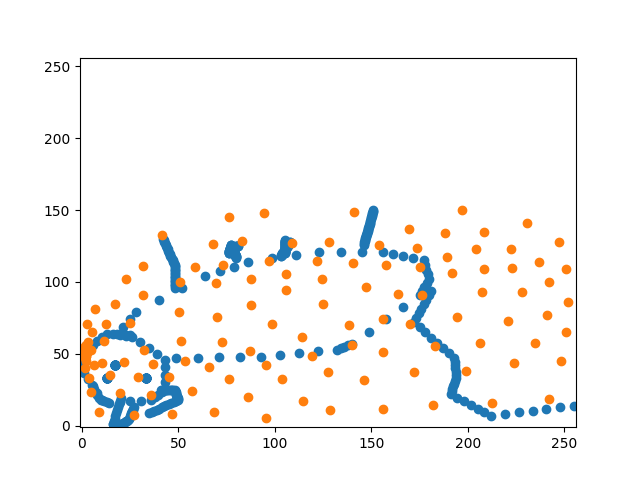
\includegraphics[keepaspectratio, scale=0.45]{draw-forecast/fig/pointnet_output1.png}
    \subcaption{全データ}
    \label{fig:pointnet_output}
  \end{minipage}
  \begin{minipage}[b]{0.45\linewidth}
    \centering
    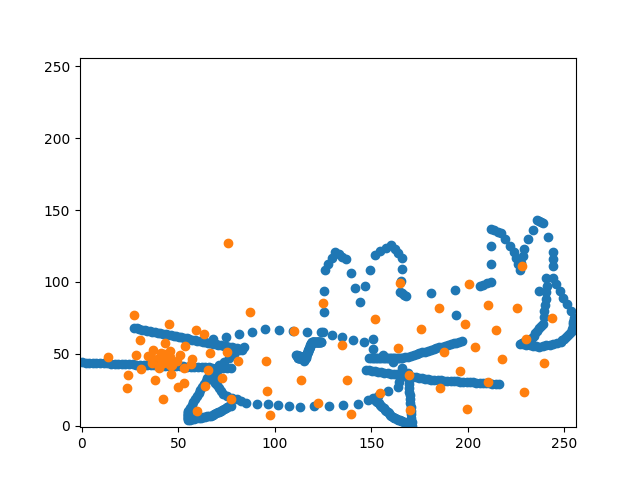
\includegraphics[keepaspectratio, scale=0.45]{draw-forecast/fig/pointnet_output2.png}
    \subcaption{Perplexityにより質を改善したデータ}
    \label{fig:pointnet_output_perplexity}
  \end{minipage}
  \caption{青が完成形・オレンジがモデルの出力}
\end{figure}

Quick Draw!\cite{quickdraw} のデータセットは、世界中のユーザーから集めたデータであるため質のばらつきが大きく、人間でも判別がつかないようなデータも多く含まれていました。このため、まずデータの選別を行う必要があると考え、PointNet\cite{pointnet}を用いたクラス分類モデルを構築し、Perplexityを用いて低品質なデータを除外しました。データセットを半分に削減した結果、図\ref{fig:pointnet_output_perplexity}のように生成された点群に多少のまとまりが見られるようになりましたが、それでも絵としての復元には至りませんでした。

\subsection{失敗した要因}
クラスの分類タスクでは、PointNet\cite{pointnet}を用いたモデルが80\%以上の精度を達成したことから、点群によるアプローチが上手くいかなかった原因はエンコーダではなくデコーダにあると考えられます。固定長を一度に出力する手法では点群の順序に依存しない特性、逐次生成ではデータ内のの描き順のばらつきによる一貫性の欠如が、上手く生成できなかった原因であると思います。

\section{時系列データ}
Quick, Draw!\cite{quickdraw}のデータは、点の座標の時系列データとして表現されているため、まず単純なTransformerを用いて次の点を予測する学習を試みましたが、意味のある出力を得ることはできませんでした。

Quick Draw!\cite{quickdraw}のデータセットを用いた線画の生成に関する論文として、sketchRNN\cite{sketchRNN}というモデルがあり、Googleが開発した初めのモデルとなります。sketchRNN\cite{sketchRNN}は、エンコーダに双方向性LSTMを採用し、入力データを潜在空間に埋め込んだ後、デコーダとしてLSTMを用いて復元する、VAEに基づいた生成モデルです。
\begin{figure}[h]
  \centering
  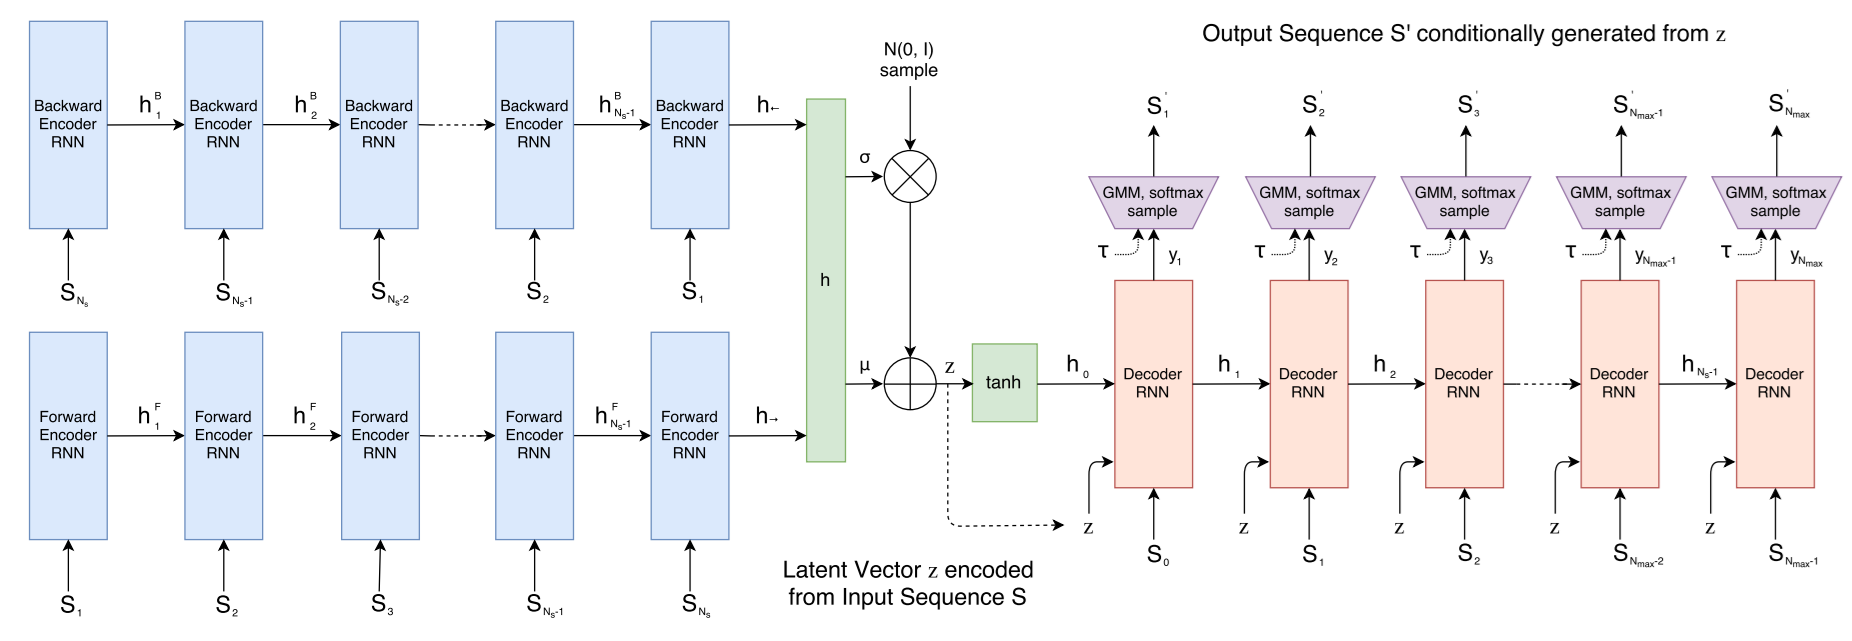
\includegraphics[scale=0.45]{draw-forecast/fig/sketchrnn.png}
  \caption{SketchRNN}
  \label{fig:sketchrnn}
\end{figure}
データの前処理として、直接的な座標ではなく前の点からの差分の座標を使用し、「ペンを下ろしている」・「ストロークの終わり」・「絵の終わり」の3つの状態を表すワンホットベクトルを合わせた5次元の系列データで学習を行います。出力については、座標の差分の分布に混合正規分布を仮定し、サンプリングによって次点の予測を行います。混合正規分布を用いることで、複数の書き順が存在することによって学習が不安定化する問題点を解決しています。ただし、複数のクラスを1つのモデルで同時に学習させることは難しく、1クラス毎に個別のモデルを学習させる必要があります。

また、LSTMではなくTransformerを用いたsketchformer\cite{sketchformer}というモデルもあり、こちらのモデルではsketchRNN\cite{sketchRNN}とは異なり、単一モデルで複数クラス全ての学習を同時に行っても精度よく生成することが可能となります。しかし、論文の内容を再現してみても学習が上手く進まず、時間の制約から本プロジェクトでは使用することができませんでした。

\section{終わりに}

今回は、途中まで描かれた絵から完成形を描くAIの作成に挑戦しましたが、時間の制約と実力不足により、最終的には初期の線画生成モデルであるSketchRNN\cite{sketchRNN}を採用する形となり、Transformerを用いたsketchformer\cite{sketchformer}などの新しいモデルや、独自の工夫を加えた実験を十分に行うことができずに終わってしまいました。今後は、sketchformer\cite{sketchformer}の実装や、Diffusionモデルなどの様々な生成手法を取り入れた実験を行い、より完成度の高いモデルを作成していきたいと思います。


\bibliographystyle{junsrt}
\bibliography{
    line-tracer/line-tracer,
    eye-track-cursor/eye-track-cursor,
    moving-kaira-kun/moving-kaira-kun,
    no-lose-janken/no-lose-janken,
    syllabus-rag/syllabus-rag-miyamae,
    syllabus-rag/syllabus-rag-kambara,
    draw-forecast/draw-forecast
}
\nocite{*}

\chapter*{本会誌について}
\section*{執筆者}
\subparagraph*{第\ref{chap:line-tracer}章:カメラ入力を用いた強化学習によるライントレーサの実現}
平塚謙良
\subparagraph*{第\ref{chap:eye-track-cursor}章:目線で操るマウスカーソル}
稲葉陽孔
\subparagraph*{第\ref{chap:moving-kaira-kun}章:KaiRAくんを動かそう}
岡本和優
\subparagraph*{第\ref{chap:no-lose-janken}章:最強じゃんけんAI}
千葉一世
\subparagraph*{第\ref{chap:syllabus-rag-overview}章:京大シラバス検索RAGシステム - システム概要編}
宮前明生
\subparagraph*{第\ref{chap:syllabus-rag-search}章:京大シラバス検索RAGシステム - 検索手法編}
神原みちる
\subparagraph*{第\ref{chap:draw-forecast}章:お絵描き予測AI}
千葉一世


\section*{京都大学人工知能研究会KaiRA}
\subparagraph*{代  表} 松田拓巳
\subparagraph*{活動日時} 毎週木曜日 18:30〜
\subparagraph*{活動場所} 文学部教室・株式会社Deepcraft\ 京都オフィス(百万遍ビル3F)など
\subparagraph*{入会資格} 大学、学部、回生問わず、AIに興味がある方
\subparagraph*{会  費} 無料
\subparagraph*{活動内容} 機械学習に関する本の輪読会、コード読み・実装会、kaggleへの参加など


\begin{table}[b]
	\centering
	\begin{tabular}{lcll}
		\multicolumn{4}{c}{ {\LARGE 会誌 vol.8} }	\\
		\bhline{1pt}
		発行日 && 2024年11月吉日 初版発行&\\
		発行 && 京都大学人工知能研究会KaiRA&\\
		公式サイト && \url{https://kyoto-kaira.github.io/}&\\
    メールアドレス && \url{kyoto.kaira@gmail.com}&\\
		X(旧Twitter) && \url{https://x.com/kyoto_kaira}&\\
		\bhline{1pt}
	\end{tabular}
\end{table}

\end{document}



